pc\documentclass[a4paper,12pt,openany]{book}
\usepackage{layout}
\usepackage[utf8]{inputenc}
\usepackage[left=1.5cm,top=2.5cm,right=1.5cm,bottom=2.5cm]{geometry} 
\usepackage[spanish, es-tabla]{babel}
\renewcommand{\baselinestretch}{1.5}
\usepackage{cite} % para contraer referencias
\usepackage{geometry}
\geometry{bindingoffset=2cm}
\usepackage{color}
\usepackage{graphicx}
\usepackage{epsfig}
\usepackage{multirow}
\usepackage{colortbl}
\usepackage[table]{xcolor}
\usepackage{float}
\usepackage{subfig}
\definecolor{lightgray}{gray}{0.9}
\usepackage{titling}
\usepackage{blindtext}
\usepackage[T1]{fontenc}
\usepackage{lmodern}
\usepackage{parskip}
\usepackage{xcolor}
\usepackage{emptypage}
\definecolor{gris}{RGB}{220,220,220}
\newcommand{\sectionbreak}{\clearpage}
\begin{document}

\begin{titlepage}
   \null\vfill
\thispagestyle{empty} 
	\centering
	\includegraphics[width=0.15\textwidth]{example-image-1x1}\par	\vspace{1cm}
   \centering
	{\scshape\LARGE Herramientas de investigación en Linea: Lo que todo Profesional exitoso debe conocer \par}
	\vspace{1cm}
	{\Large\itshape Roberto Acuña, José Manuel Gomez, Christian Caicedo\par}
	\vfill
	{\large \today\par}
\end{titlepage}
 
Dedicatoria
\tableofcontents
\chapter{Introducción}
Actualmente, los jóvenes y no tan jóvenes investigadores que inician su andadura científica se enfrentan a grandes desafíos, que en ocasiones van muchas mas allá de la profundidad de conociendo que posean en el área en que se desarrollan. más superficialmente las herramientas estadísticas necesarias para evaluar sus resultados, pero, en demasiadas ocasiones, conocen poco o nada los pasos necesarios para iniciar un trabajo de investigación, un estado de la cuestión o una revisión sistemática, iniciando el proceso de forma intuitiva y sin haber visto una metodología determinada ni las herramientas apropiadas que puedan facilitarles el trabajo. Esto hace perder mucho tiempo, tanto el propio investigador como a sus tutores, durante el inicio de la investigación del doctorando. Estos es debido a que en muchos programas o másteres de doctorado se centran demasiado en las técnicas y metodologías del área de investigación que se va a añadir pero en demasiados casos, dejan otros tipos de metodología más general, como hacer una búsqueda sistemática de artículos científicos de una temática, fuera del currículum del máster. Esto es especialmente crítico según en qué áreas de investigación se trate.

Este libro pretende convertirse en una herramienta de consulta indispensable para profesionales (informáticos, médicos, administradores de empresas, estadísticos, biólogos, etc) y estudiantes universitarios que deseen involucrarse en el campo de la investigación. El objetivo es que el investigador principiante sea capaz de realizar la búsqueda bibliográfica así como el procesamiento y la publicación de resultados a través de artículos, libros, tesis o cualquier otro tipo de documento mediante el uso de herramientas gratuitas disponibles en línea.

Sin lugar a dudas, podemos decir que vivimos en la era digital, también conocida como la era de las \textbf{tecnologías de la información y comunicación} (TIC) en una especie de aldea global que nos interconecta a todos los seres humanos del planeta. Lo cierto es que, gracias a los sistemas de telecomunicación actuales, somos los seres humanos con el mayor acceso a la información de la historia. Para lograr esto las computadoras e Internet han jugado un papel determinante y han hecho posible que exista una gran cantidad de herramientas tecnológicas que están disponibles para facilitar nuestras tareas, situación que debemos aprovechar para alcanzar ventajas competitivas y convertirnos en profesionales del futuro: competentes, autónomos, desarrolladores de competencias esenciales como pensamiento sistémico, capacidad de crear, de cuestionar, trabajar en equipo, con la finalidad de buscar y encontrar soluciones como en la vida real.

Algo que las personas deben conocer es que no toda la información disponible en la Web es verídica, como tampoco no toda es de calidad. ¿Qué hacer entonces con la avalancha de información que encontramos con solo ubicar un tema en la barra de búsqueda de Google, Bing, YouTube o cualquier otro buscador para que muestre una lista de sitios en linea que contienen información relacionada con el tema que buscamos? ¿Cómo saber si es correcta esa información? La respuesta a estas preguntas no es trivial, nos tocará discernir por nosotros mismos la calidad y veracidad de la información, lo que, seguramente, tendrá un precio muy alto en tiempo o, incluso, nos puede llevar a trabajar con información equivocada. Después de leer cientos o miles de artículos en mi vida investigadora, he podido leer lamentables artículos que incumplen con las más elementales reglas de una publicación científica, como no justificar una contundente afirmación con datos ni con una referencia apropiada, o no citar una fuente primaria.

Para encontrar información cualificada y de calidad hay que ir a los lugares adecuados. Pero incluso en estos sitios, debemos ser capaces de discernir un buen artículo de uno malo o con errores. Esto lo tenemos que tener en cuenta tanto para la investigación como en nuestra vida cotidiana. Por ejemplo, si un tema te gusta, inicialmente puedes realizar una búsqueda superficial en cualquier buscador como Google o Bing, a continuación puedes buscar vídeos en YouTube y cuando ya tengas al menos una idea básica puedes tomar un curso en linea, para ello en la actualidad existen los cursos MOOC en plataformas como Miriadax\footnote{https://miriadax.net/home}, Edx\footnote{https://www.edx.org/es}, Coursera\footnote{https://www.coursera.org} entre otros muchos, los cuales son patrocinados por universidades o instituciones particulares y con los cuales te adentraras muy rápido en el tema que intentas investigar, seguidamente podrás buscar mas información de calidad en google Académico\footnote{https://scholar.google.es} y en bases de conocimiento especializadas como Scopus\footnote{https://scopus.com}, Wed of Science\footnote{https://clarivate.com/products/web-of-science}, IEEE\footnote{https://https://ieee.org}, entre otras, en las cuales los resultados de la búsqueda, nos llevan a artículos científicos y libros, siendo esta información, a priori, de calidad valida para nuestro proceso de investigación. Hay que dejar claro que para poder tener acceso a muchos  artículos y libros debes pagar las suscripciones a las diferentes bases de datos o pertencer a una institución educativa que haya pagado previamente este acceso o solicitarles a las autoridades académicas que adquieran suscripciones institucionales a éstas. Se recomienda al menos \textbf{Scopus}, ya que es la bases de conocimiento con revistas de mayor prestigio del mundo.

Una vez que ya estés inmerso en este mundo del conocimiento, el siguiente paso es conocer una serie de herramientas que te ayuden en tu proceso de investigación. Hay que tomar en cuenta que mucha de la información esta en inglés, por lo que si no no tienes al menos un nivel adecuado de compresión lectora, será el momento adecuado de iniciar en paralelo un curso en este idioma, para ello recomendamos que tomes cursos en academias locales, o utilices herramientas gratuitas o de pago disponibles es la web.

Actualmente hay muchas herramientas en linea para procesos de investigación, de las cuales en base a nuestra experiencia hemos seleccionado algunas que nos han ayudado a nosotros y seguro te ayudaran a ti, entre las principales aplicaciones que  estudiaremos en los diferentes capítulos de este libro están Parsifal\footnote{https://parsif.al}, Mendeley \footnote{https://www.mendeley.com}, y Overleaf \footnote{https://www.overleaf.com}, todas ellas de carácter on line, que a mas de ayudarte en la documentación de tu investigación te permitirá trabajar con otras personas de manera colaborativa\footnote{Varias personas pueden trabajar simultáneamente en un mismo documento},  cabe indicar que todas ellas están interrelacionadas entre si y que al final terminaras utilizándolas en su conjunto. 

\chapter{Buscadores}
En este primer capitulo llegamos a nuestro primer encuentro con la información y es el sitio web de google\footnote{https://www.google.com/} el buscador mas utilizado del mundo, el cual de seguro te resulta familiar y has utilizado, ya en el sitio solo tendrás que escribir en la barra de dirección una pregunta relacionada con la información que desean encontrar. 

\begin{figure}[ht]
  \centering
	
\includegraphics[width=10cm]{google1.png}
\caption{Navegador de Google}
  \label{fig:google1}
\end{figure}

Aquí en la barra de búsqueda luego de escribir la pregunta acerca de la información que deseas encontrar, google te mostrara una lista de documentos encontrados, a los cuales podrás acceder simplemente con realizar un clic sobre la linea que deseas y esto te llevara al documento seleccionado. No  entraremos en mayores detalle en esta parte pues todo el mundo a realizado alguna consulta alguna vez en su vida, solo diremos que deben ser lo mas explícitos posibles para alcanzara mejores resultados en su búsqueda, ahora si debes discernir entre la información que se obtiene, cual es  correcta y cual no, para su investigación.

Ahora que ya tienes una idea básica del tema que estas buscando, en muchos casos con la información encontrada sera suficiente y llenara nuestras expectativas, pero si no estas conforme con la información encontrada, debes seguir nuevos procesos de búsqueda especializada, por ello de aquí en adelante comienza nuestra aventura de encontrar información de calidad y validada, que te ayudara en tu proyecto de investigación.

En la siguiente tabla \ref{tabla:infor1}, presentamos varios sitios que contienen información importante, los cuales no abarcaremos en este libro, pero que seguramente te pueden ser de mucha valía, en tu proceso de búsqueda de información de calidad, los cuales te podrán servir para el desarrollo de tus trabajos escolares o procesos de investigación que realicemos.

\begin{table}[ht]
\begin{center}
\begin{tabular}{ | m{6 cm} | m{10 cm}| }
\hline
\rowcolor[cmyk]{1,1,0,0} {\textcolor{white}{\centering SITIO WEB}} & {\textcolor{white}{\centering {\centering INFORMACIÓN}} \\ \hline 

We Are Social  & Sitio web con estadísticas relacionadas con la utilización del internet por parte de la población mundial.  \\ \hline
Statista  & Sitio web con estadísticas relacionadas con la utilización del internet por parte de la población mundial.  \\ \hline
Wordreference & Diccionario de Idiomas en linea.\\ \hline
GeoNames & Base de datos geográfica Geonombres cubre todos los países y contiene más de ocho millones de nombres de lugares que están disponibles para su descarga gratuita.  \\ \hline
Netblocks & Sitio de estadísticas de Internet.  \\ \hline
Prezi & Sitio de creación de diapositivas.  \\ \hline
Betterment & Banco virtual.  \\ \hline
Forvo & Pronunciación de tolas las palabra del mundo. \\ \hline
\end{tabular}
\caption{Lista de sitios con información interesante}
\label{tabla:infor1}
\end{center}
\end{table} 

\subsection{Youtube}

\begin{figure}[ht]
  \centering
	
\includegraphics[width=8cm]{youtube2.png}
\caption{Youtube}
  \label{fig:youtube2}
\end{figure}

Otra opción que debe explorarse en la búsqueda de información, son los vídeos y para ello la herramienta mas popular y conocida es youtube\footnote{https://www.youtube.com/}, sitio al que al igual que hiciste en google, bastara con escribir en su barra de búsqueda la pregunta acerca de la información que quieras encontrar y dar clic, nuevamente tendrás una lista de opciones de vídeos que puedes ver y a discernir entre la información resultante.

\begin{figure}[ht]
  \centering
	
\includegraphics[width=14cm]{youtube1.png}
\caption{Navegador de Youtube}
  \label{fig:youtube1}
\end{figure}

Como experiencia personal puedo asegurar que muchas veces encontramos vídeos, que explican muy bien la temática que estas buscando y aclaran de una manera óptima la temática que buscas, conocimiento que luego podrás aplicar en tu investigación o hacerlo parte de tu conocimiento general.   

Youtube a mas de ser un sitio que contiene vídeos especializados en diferentes áreas del conocimiento subidos por youtubers, contiene una variedad de películas, programas de televisión, vídeos musicales contenido amateur como videoblogs y youtube Gaming. La manera en que los usuarios de youtube muchas veces podemos acceder a la información que comparten los youtubers, es a través de los canales, a los cuales podemos suscribirnos si nos parecen interesantes. En la siguiente tabla \ref{tabla:tabYou}, presentamos varios canales que nos parecen interesantes.

\begin{table}[ht]
\begin{center}
%\begin{tabular}{|l >{\centering\arraybackslash}m{4cm} |l >{\centering\arraybackslash}m{8.5cm}|l}
%\begin{tabular}{| >{\arraybackslash}m{6cm}|>{\arraybackslash}m{10 cm} |}

\begin{tabular}{| m{6 cm}| m{10 cm} |}
\hline
\rowcolor[cmyk]{1,1,0,0} {\textcolor{white}{\centering CANAL}} & {\textcolor{white}{\centering {\centering INFORMACIÓN}} \\ \hline 
English In The Spotlight & Canal de enseñanza del idiomas Ingles.\\ \hline
A Smart Code & Canal dedicado a la programación.  \\ \hline
Aprende con Alf & Canal dedicado a la programación y estadistica.  \\ \hline
The Tabernacle Choir at Temple Square  & Canal con musica espiritual.  \\ \hline
Tus Clases de Portugués & Canal que te enseña el idioma portugués desde cero.  \\ \hline
\end{tabular}
\caption{Lista de canales de YouTube, interesantes}
\label{tabla:tabYou}
\end{center}
\end{table} 

\chapter{Cursos MOOC}
 
Este nuevo capitulo te fascinara, pues ahora que ya tienes conocimiento acerca de tu tema de investigación con información cualificada, esto te pondrá a un nivel en el que te darás cuenta que necesitas una serie de nuevos conocimientos actualizados y de calidad para vincularlos a tu investigación y para ello encontraras un buen recurso en los cursos masivos en linea MOOC\footnote{Acrónimo en Ingles de Massive Online Open Courses}, los cuales son la nueva forma en que las \textbf{universidades del Mundo se vinculan con la sociedad} y es un formato con el que muchas empresas también están incursionando en el mundo de la educación. En la gráfica \ref{imagen:plataformas} puedes ver imágenes iniciales de plataformas MOOC. \

\begin{figure}[ht]
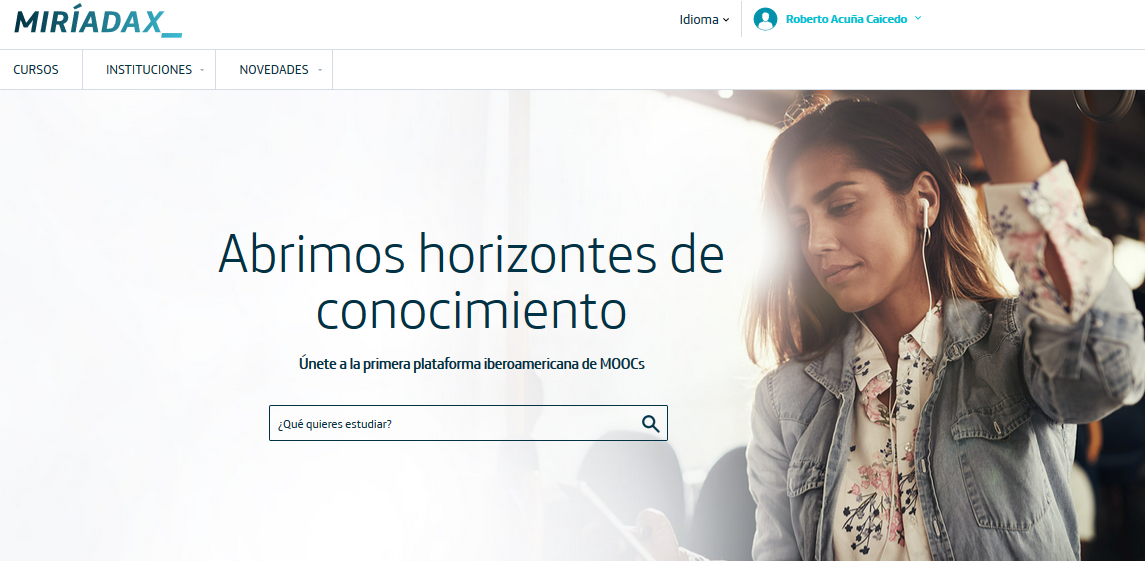
\includegraphics[width=5cm]{miriada1}

\includegraphics[width=5cm]{edx1}
\centering
\\
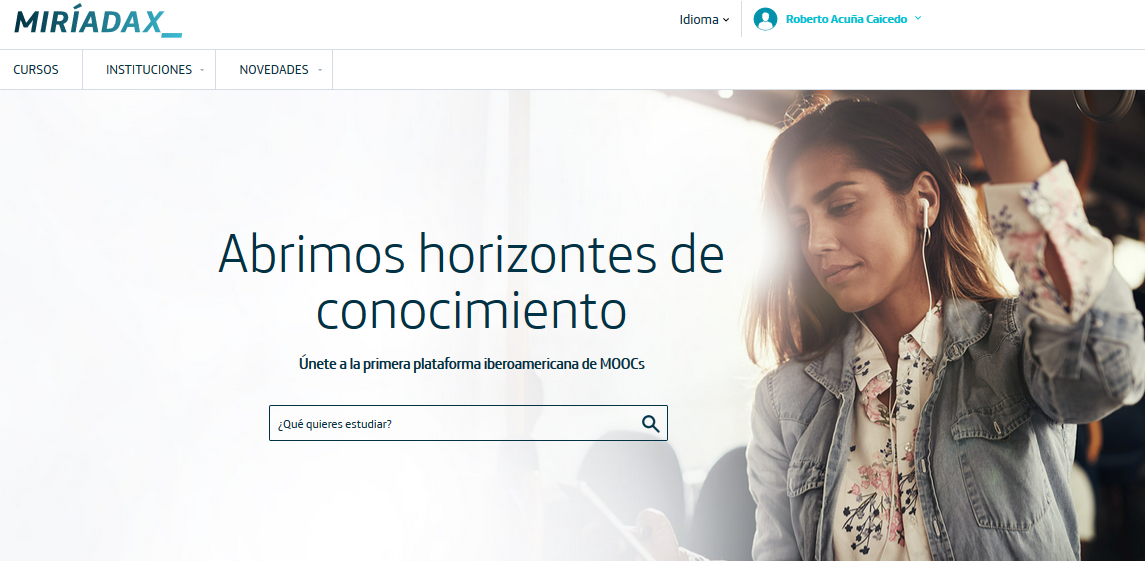
\includegraphics[width=5cm]{miriada1}
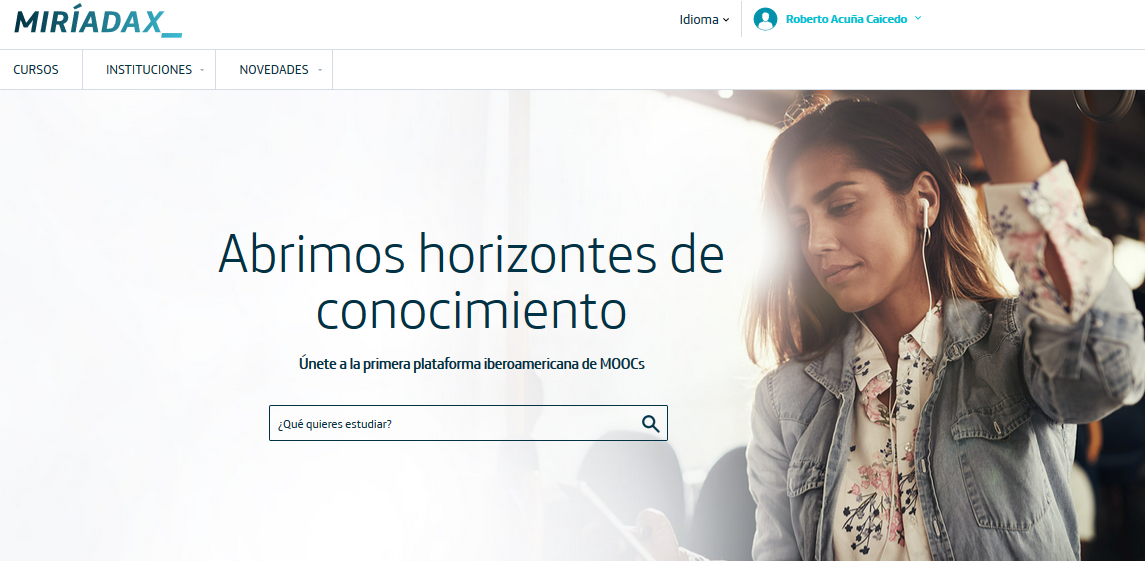
\includegraphics[width=5cm]{miriada1}
\centering
\caption{Plataformas MOOC}
\label{imagen:plataformas}
\end{figure}

Los cursos MOOC tienen las siguientes características:

\begin{itemize}
\item Son dictados en plataformas en linea por universidades o empresas, con el fin de brindar conocimiento al mundo.
\item Cursos gratuitos y de pago, también existen plataforma que tienen ambas opciones y el usuario escoge dependiendo de los servicios que quiera tener.
\item Calidad y variedad de áreas de conocimiento abarcadas.
\item Puedes estudiar los cursos que quieras, cuando quieras y donde quieras con solo acceder a la plataforma a través de su App o su sitio web.
\end{itemize}

Además de las características descritas, otra ventaja de los cursos MOOC, es que son respaldados por instituciones de prestigio mundial, te imaginas tener certificaciones en tu hoja de vida otorgadas por universidades como Massachusetts Institute of Tecnology, Stanford, Harvard, Politécnica de Madrid, Politécnica de Valencia, Universidad de Alicante, Escuela Superior Politécnica del Ecuador, Pontificia Universidad Católica del Perú entre otras muchas universidades de prestigio, ademas de cursos dictados por empresas como telefónica, Microsoft, etc,. entre las principales plataformas de cursos están: 

\section{Miriadax}

MiriadaX, principal plataforma de cursos web en iberoamerica y la primera en el mundo en habla no inglesa, nació como una iniciativa conjunta entre Telefónica Educación Digital y Banco Santander, cuenta a mayo del 2018 con mas de 4 millones de suscriptores y mas de 100 partners\footnote{Socios} educativos. Los cursos que se dictan en esta plataforma se encuentran principalmente en idioma español, varios en portugués y unos pocos en idioma ingles. Estos cursos pueden ser tomados por los usuarios registrados y se accede por medio de  un navegador Web, con solo escribir en su barra de búsqueda, la dirección web \footnote{https://miriadax.net}, o a través de su app en los dispositivos móviles. Al acceder a la plataforma veremos primeramente la pantalla de inicio, la cual vemos en la figura \ref{fig:miriada1}. 

\begin{figure}[ht]
  \centering
	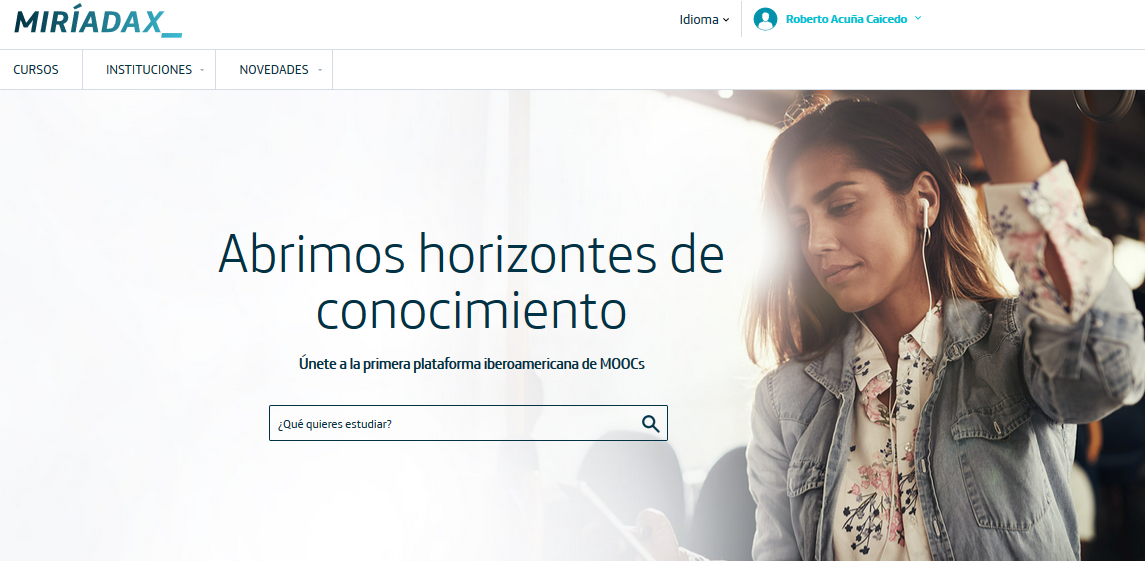
\includegraphics[width=10cm]{miriada1.png}
\caption{Miriadax Principal Plataforma de cursos MOOC de Iberoamerica}
  \label{fig:miriada1}
\end{figure}

Una vez que estemos en la pagina principal de miriadax, usted podrá explorar toda la plataforma de cursos, tal como se presentan en la figura \ref{fig:miriada2}, 

\begin{figure}[ht]
  \centering
	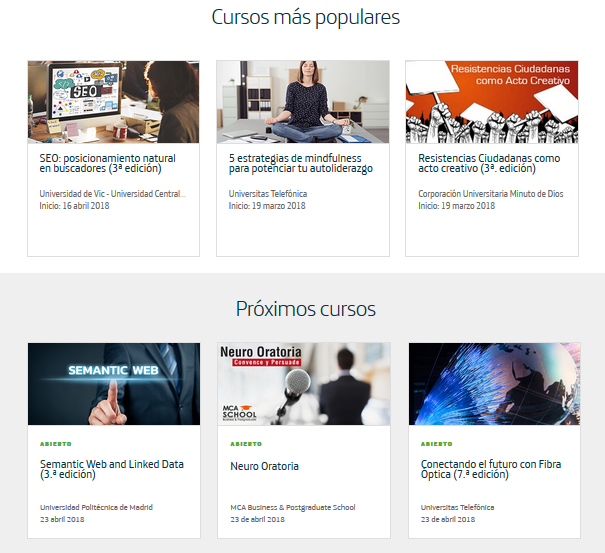
\includegraphics[width=10cm]{miriada2.png}
\caption{Cursos disponibles en Miridax}
  \label{fig:miriada2}
\end{figure}

Hay que tener en cuenta que debemos registrarnos en esta plataforma para poder acceder a los cursos que se desarrollan en ella, esto lo realizamos dando clic en la opción de \textbf{REGÍSTRATE} en la parte superior de la pantalla tal como se ve en la figura \ref{fig:miriada3}, para a continuación registramos tal como vemos en la figura \ref{fig:miriada7}. Cuando ya tengamos una cuenta solo debemos identificarnos, esto lo podemos realizar dando  clic en la opción de \textbf{ACCEDER} en la parte superior de la pantalla e ingresando a continuación nuestro usuario y contraseña. 

\begin{figure}[ht]
  \centering
	
\includegraphics[width=10cm]{miriada3.png}
\caption{Acceso a Registrase en Miriadax}
  \label{fig:miriada3}
\end{figure}

\begin{figure}[ht]
  \centering
	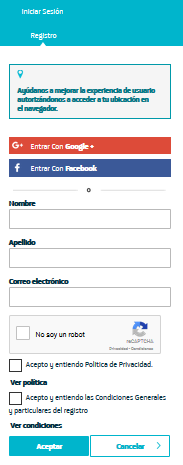
\includegraphics[width=5cm]{miriada7.png}
\caption{Registrarse en Miriadax}
  \label{fig:miriada7}
\end{figure}

Una vez que estemos debidamente registrados, podemos navegar en la plataforma y buscar el curso o cursos de nuestra preferencia, esto lo realizamos con solo seleccionar su imagen dando clic sobre este, lo que nos permitirá acceder al mismo. Una vez dentro del curso, en la parte inicial podemos ver su vídeo promocional tal como se muestra en la figura \ref{fig:miriada4}, el cual nos dará una idea general de las temáticas a tratarse, luego de lo cual podemos discernir si nos interesa o no. 

\begin{figure}[ht]
  \centering
	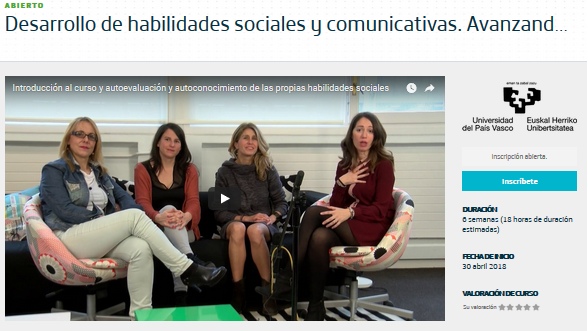
\includegraphics[width=8cm]{miriada4.png}
\caption{Acceder a los cursos en Miriadax}
  \label{fig:miriada4}
\end{figure}

Miriadax, organiza cada uno de sus cursos mediante módulos, los cuales tienen un tiempo especifico de duración, que por lo general es de una semana. En cada modulo los estudiante deberán desarrollar las siguiente actividades:

\begin{itemize}
\item Revisar el material escrito, audiovisual.
\item Desarrollar tareas.
\item Rendir evaluaciones.
\end{itemize}

Finalmente si culminamos el curso podrás obtener dos tipos de certificados:

\begin{itemize}
\item \textbf{Certificado de participación}: Es gratuito, se consigue cuando el alumno a superado el 75\% de los módulos del curso. Con este certificado \textbf{Miriadax} reconoce la participación del alumno en un curso, se lo puede descargar como un archivo pdf o un badge, que se muestra en la plataforma y puede exportarse a mozilla open. Figura \ref{fig:miriada8}.  

\begin{figure}[ht]
  \centering
	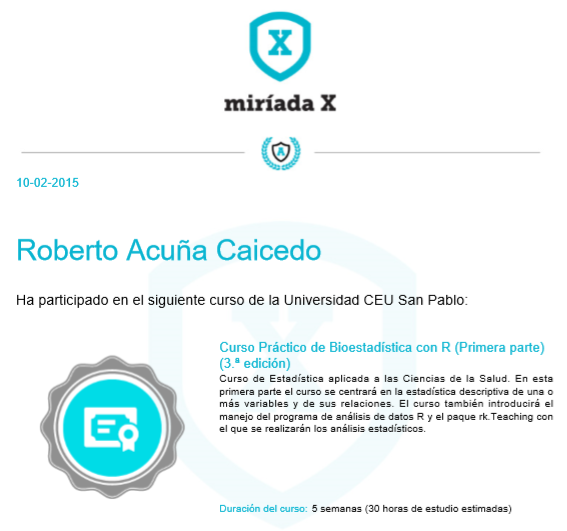
\includegraphics[width=10cm]{miriada8.png}
\caption{Certificado de participación Miriadax}
  \label{fig:miriada8}
\end{figure}

\item \textbf{Certificado Digital de Superación}: Es de pago, se consigue cuando el alumno a superado el 100\% de los módulos del curso. Con este certificado \textbf{Miriadax} y la \textbf{entidad educativa que dicta el curso}, previo al pago de 40 euros, reconocen la participación del alumno en un curso, se lo puede descargar como un archivo pdf o un badge, que se muestra en la plataforma y puede exportarse a mozilla open. Figura \ref{fig:miriada9}

\begin{figure}[ht]
  \centering
	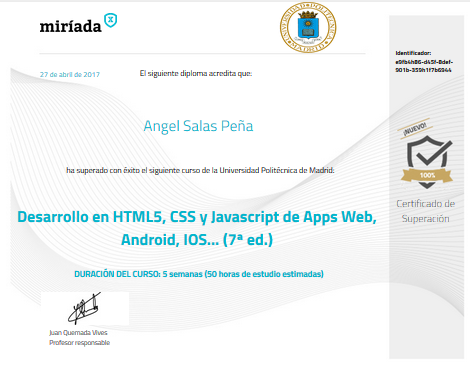
\includegraphics[width=10cm]{miriada9.png}
\caption{Certificado de Superación Miriadax}
  \label{fig:miriada9}
\end{figure}
\end{itemize}

\clearpage
\subsection{Universidades e instituciones que forman parte de miriadax}

Las universidades e instituciones que forman parte de miriadax y que constantemente publican cursos MOOC, en esta plataforma son:

\begin{figure}[ht]
  \centering
	
\includegraphics[width=10cm]{miriada10-1.png}
\caption{universidades e instituciones que forman parte de Miriadax}
  \label{fig:miriada10-1}
\end{figure}

\begin{figure}[ht]
  \centering
	
\includegraphics[width=10cm]{miriada10-2.png}
\caption{universidades e instituciones que forman parte de Miriadax}
  \label{fig:miriada10-2}
\end{figure}

\begin{figure}[ht]
  \centering
	
\includegraphics[width=10cm]{miriada10-3.png}
\caption{universidades e instituciones que forman parte de Miriadax}
  \label{fig:miriada10-3}
\end{figure}

\begin{figure}[ht]
  \centering
	
\includegraphics[width=10cm]{miriada10-4.png}
\caption{universidades e instituciones que forman parte de Miriadax}
  \label{fig:miriada10-4}
\end{figure}

\begin{figure}[ht]
  \centering
	
\includegraphics[width=10cm]{miriada10-5.png}
\caption{universidades e instituciones que forman parte de Miriadax}
  \label{fig:miriada10-5}
\end{figure}

\begin{figure}[ht]
  \centering
	
\includegraphics[width=10cm]{miriada10-6.png}
\caption{universidades e instituciones que forman parte de Miriadax}
  \label{fig:miriada10-6}
\end{figure}

\clearpage
\section{Edx}

Open Edx, es la principal plataforma de cursos MOOC en idioma Ingles, reúne a las mejores universidades e instituciones del mundo, fue fundada por Harvard University y el Masachuset Institute of Tecnology en el 2012. Tiene como misión \textbf{''Incrementar el acceso a la educación de alta calidad para todos, en todas partes, mejorar la enseñanza y el aprendizaje en el campus y en linea, avanzar en la enseñanza y el aprendizaje a través de la investigación''}.  

A mayo del 2018 cuenta con mas de 130 partners educativos globales. Los cursos que se dictan en esta plataforma se encuentran principalmente en idioma ingles, además dictan cursos en idioma español, portugués entre otros. Los cursos que se ofrecen en la plataforma son tomados por los usuarios registrados, a ella se accede por medio de  cualquier navegador Web con solo escribir en su barra de búsqueda, la dirección web\footnote{https://www.edx.org/es}, o a través de su app en los dispositivos móviles. Al acceder a la plataforma veremos primeramente la pantalla de inicio, la cual vemos en la figura \ref{fig:edx1}

\begin{figure}[ht]
  \centering
	
\includegraphics[width=10cm]{edx1.png}
\caption{Edx Pagina principal}
  \label{fig:edx1}
\end{figure}

Una vez que estemos en la pagina principal de \textbf{Edx}, usted podrá explorar toda la plataforma de cursos, tal como se presentan en la figura \ref{fig:edx2}, 

\begin{figure}[ht]
  \centering
	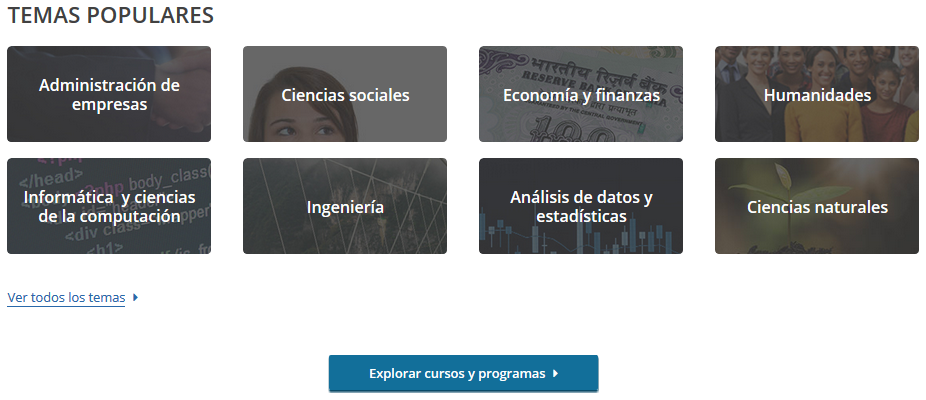
\includegraphics[width=10cm]{edx2.png}
\caption{Cursos disponibles en Edx}
  \label{fig:edx2}
\end{figure}

En esta plataforma educativa también es obligatorio registrarnos, para poder acceder a los diferentes cursos que se dictan en la plataforma, esto lo podemos realizar en la parte superior de la pantalla tal como podemos ver en las figuras \ref{fig:edx3},  \ref{fig:edx4}.

\begin{figure}[H]
  \centering
	
\includegraphics[width=10cm]{edx.png}
\caption{Acceso a Registrase en Miriadax}
  \label{fig:edx3}
\end{figure}

\begin{figure}[H]
  \centering
	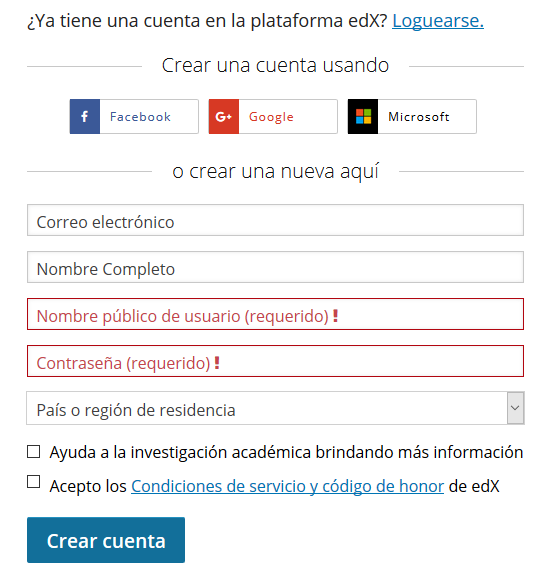
\includegraphics[width=10cm]{edx3.png}
\caption{Registrarse en Edx}
  \label{fig:edx4}
\end{figure}

 Una vez que estemos registrados, simplemente debemos, en la parte superior de la pagina web, hacemos clic en el icono \textbf{Sign In} tal como vemos en las figura \ref{fig:edx5}, luego de lo cual puede acceder a los cursos de su preferencia.

\begin{figure}[H]
  \centering
	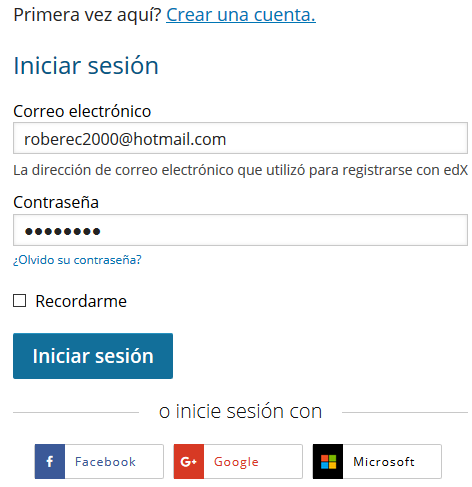
\includegraphics[width=8cm]{edx4.png}
\caption{Acceso de usuarios registrado en Edx}
  \label{fig:edx5}
\end{figure}

Para poder escoger el curso de nuestra preferencia tal como vemos en la figura \ref{fig:edx2}, solo basta con realizar un clic sobre la imagen del curso y nos llevara a la pagina de información del mismo, luego de lo cual si nos interesa podemos unirnos al curso, tal como vemos en la figura \ref{fig:edx6}.\

\begin{figure}[ht]
  \centering
	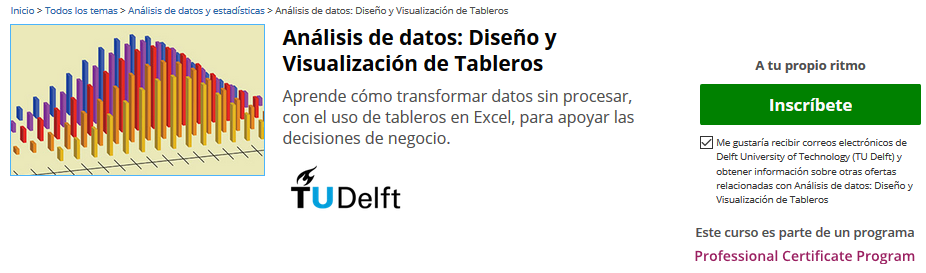
\includegraphics[width=8cm]{edx11.png}
\caption{Acceder a los cursos en Edx}
  \label{fig:edx6}
\end{figure}

Al igual que los cursos de Miriadax, cada uno de los cursos en Edx, se dividen en módulos y estos tienen un tiempo especifico de duración, que por lo general son de una semana y están perfectamente organizados, de acuerdo a lo planificado en el silabo cada estudiante deberá desarrollar lo siguiente:

\begin{itemize}
\item Revisar el material escrito, audiovisual.
\item Desarrollar tareas.
\item Rendir evaluaciones.
\end{itemize}

En la figura \ref{fig:edx12} vemos un ejemplo de la programación de un curso dictado en Edx.

\begin{figure}[ht]
  \centering
	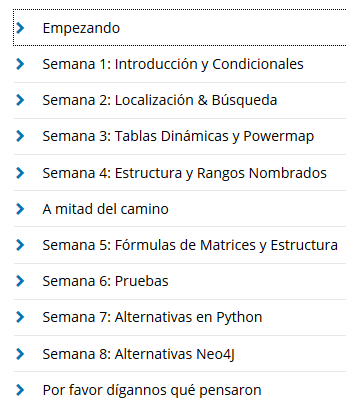
\includegraphics[width=8cm]{edx7.png}
\caption{Programación de un curso en Edx}
  \label{fig:edx12}
\end{figure}

Si tomas cursos en Edx, podrás escoger dos opciones respecto a los certificados:

\begin{itemize}
\item \textbf{Sin Certificado de participación}: Esta opción permite tomar un curso de forma gratuita, pero no proporciona ningún certificado, a pesar de obtener las notas necesarias. Figura \ref{fig:edx7}.  

\begin{figure}[ht]
  \centering
	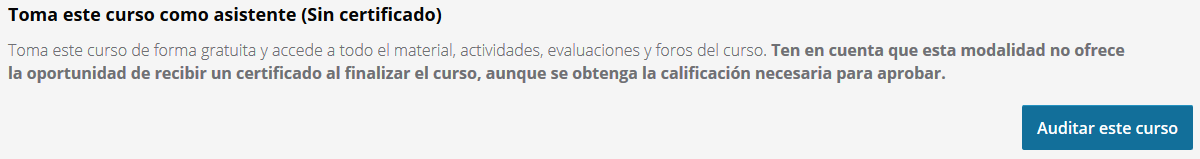
\includegraphics[width=7cm]{edx6.png}
\caption{Certificado de participación Edx}
  \label{fig:edx7}
\end{figure}

\item \textbf{Certificado Digital verificado}: Es de pago, se consigue cuando el alumno a superado el 100\% de los módulos del curso. Con este certificado \textbf{Edx} y la \textbf{entidad educativa que dicta el curso}, previo al pago de 99 dolares, reconocen la participación del alumno en un curso, se lo puede descargar como un archivo pdf en la plataforma. Figura \ref{fig:edx8}

\begin{figure}[ht]
  \centering
	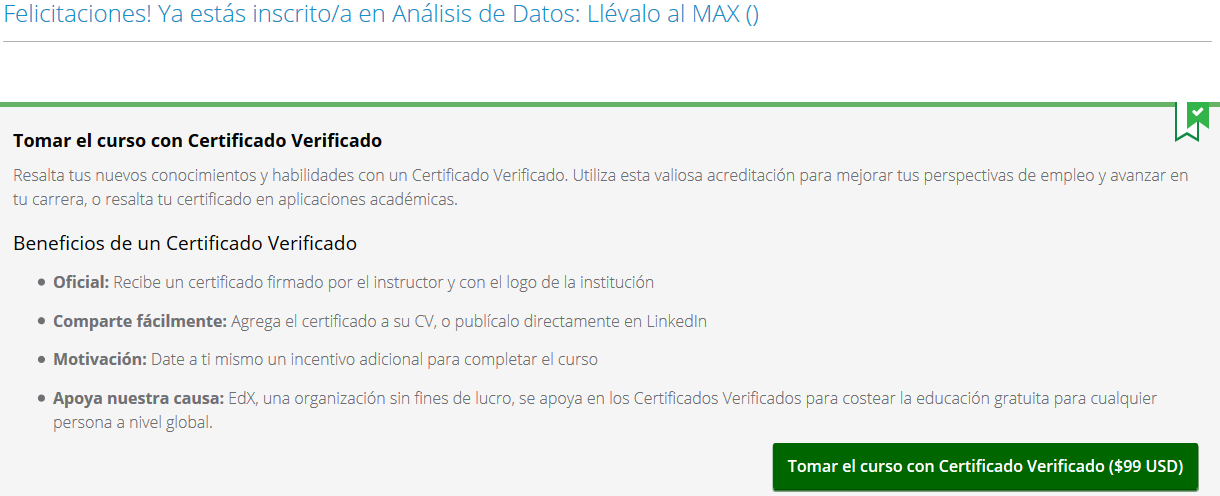
\includegraphics[width=10cm]{edx5.png}
\caption{Certificado de Superación Edx}
  \label{fig:edx8}
\end{figure}
\end{itemize}


\clearpage
\subsection{Universidades e instituciones que forman parte de Edx}

Las universidades e instituciones que forman parte de Edx y que constantemente publican cursos MOOC, en esta plataforma son:

\begin{figure}[ht]
  \centering
	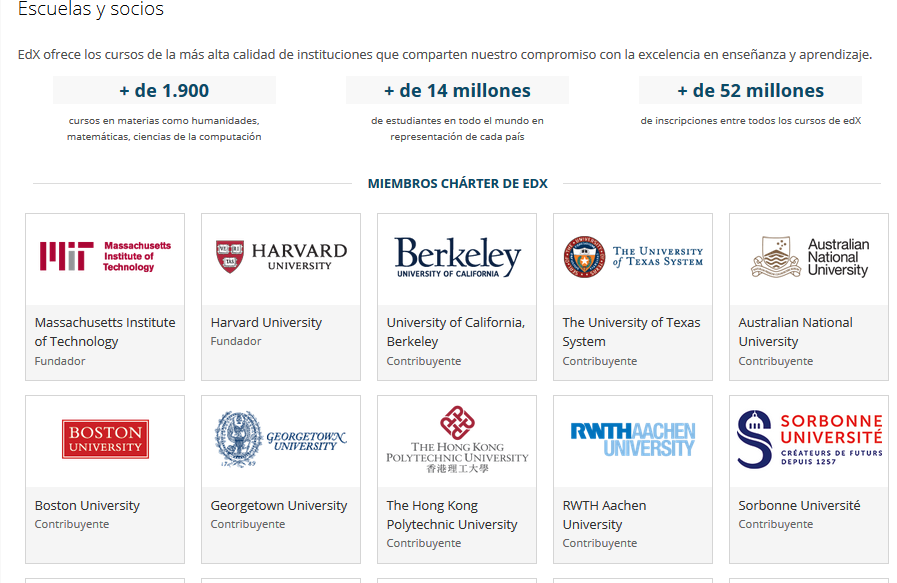
\includegraphics[width=12cm]{edx10-1.png}
\caption{universidades e instituciones que forman parte de Edx}
  \label{fig:edx10-1}
\end{figure}

\begin{figure}[ht]
  \centering
	
\includegraphics[width=12cm]{edx10-2.png}
\caption{universidades e instituciones que forman parte de Edx}
  \label{fig:edx10-2}
\end{figure}

\begin{figure}[ht]
  \centering
	
\includegraphics[width=12cm]{edx10-3.png}
\caption{universidades e instituciones que forman parte de Edx}

  \label{fig:edx10-3}
\end{figure}

\begin{figure}[ht]
  \centering
	
\includegraphics[width=12cm]{edx10-4.png}
\caption{universidades e instituciones que forman parte de Edx}
  \label{fig:edx10-4}
\end{figure}

\begin{figure}[ht]
  \centering
	
\includegraphics[width=12cm]{edx10-5.png}
\caption{universidades e instituciones que forman parte de Edx}
  \label{fig:edx10-5}
\end{figure}

\begin{figure}[ht]
  \centering
	
\includegraphics[width=12cm]{edx10-6.png}
\caption{universidades e instituciones que forman parte de Edx}
  \label{fig:edx10-6}
\end{figure}

\begin{figure}[ht]
  \centering
	
\includegraphics[width=12cm]{edx10-7.png}
\caption{universidades e instituciones que forman parte de Edx}
  \label{fig:edx10-7}
\end{figure}

\begin{figure}[ht]
  \centering
	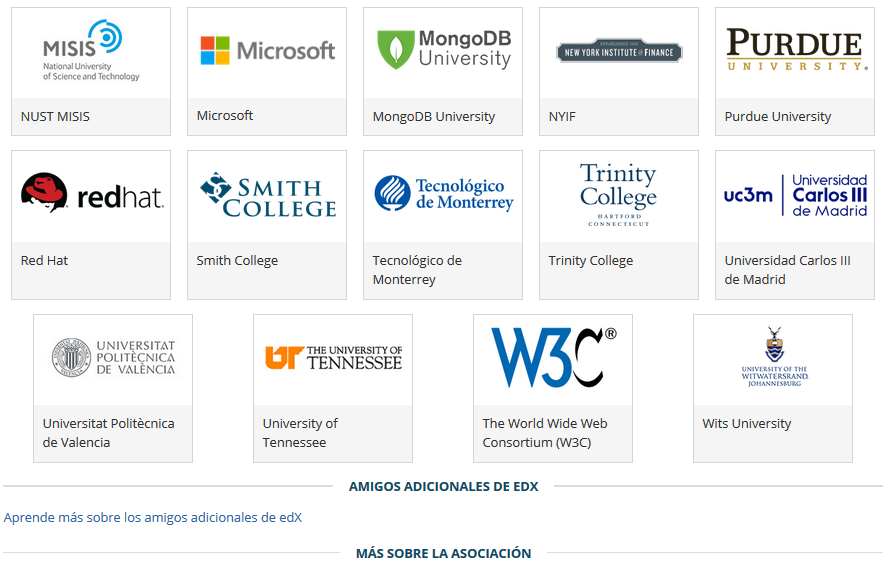
\includegraphics[width=12cm]{edx10-8.png}
\caption{universidades e instituciones que forman parte de Edx}
  \label{fig:edx10-8}
\end{figure}


\clearpage

\section{Coursera}

Coursera, es otra de las principales plataformas de cursos MOOC en la Web, cuenta a mayo del 2018, con 165 partners educativos globales. fue fundada por 2 profesores de Stanford Computer Science en el 2012, Daphne Koller and Andrew Ng. Tiene como misión, \textbf{Un mundo donde cualquier persona, en cualquier lugar, puede transformar su vida accediendo a la mejor experiencia de aprendizaje del mundo}.   

Los cursos que se dictan en esta plataforma se encuentran en idiomas ingles, español, portugués entre otros. Actualmente coursera ofrece en su plataforma mas de 2800 cursos, los cuales puedes ser tomados por los usuarios registrados, cabe indicar que el proceso de registro y acceso a la plataforma Coursera, es similar a las de Miriadax y Edx. A este sitio web accedemos por medio de  cualquier navegador Web, con solo escribir en la barra de búsqueda, su dirección web \footnote{https://www.coursera.org}, o a través de su app en los dispositivos móviles. Al acceder a la plataforma veras primeramente la pantalla de inicio, tal como ves en la figura \ref{fig:coursera1}

\begin{figure}[ht]
  \centering
	
\includegraphics[width=10cm]{coursera1.png}
\caption{Coursera Pagina principal}
  \label{fig:coursera1}
\end{figure}

Para poder escoger el curso de tu preferencia, solo basta con realizar un clic sobre la imagen del curso, tal como vemos en la figura \ref{fig:coursera2} y esto nos llevara a la pagina de información del mismo, luego de lo cual si nos interesa podemos unirnos al mismo.

\begin{figure}[H]
  \centering
	
\includegraphics[width=10cm]{coursera-cursos.png}
\caption{Cursos disponibles en Coursera}
  \label{fig:coursera2}
\end{figure}


\clearpage
\subsection{Universidades e instituciones que forman parte de Coursera}

Las universidades e instituciones que forman parte de Coursera y que constantemente publican cursos MOOC, en esta plataforma son:

\begin{figure}[H]
  \centering
	
\includegraphics[width=10cm]{coursera10-1.png}
\caption{universidades e instituciones que forman parte de Coursera}
  \label{fig:cour10-1}
\end{figure}

\begin{figure}[H]
  \centering
	
\includegraphics[width=10cm]{coursera10-2.png}
\caption{universidades e instituciones que forman parte de Coursera}
  \label{fig:cour10-2}
\end{figure}

\begin{figure}[H]
  \centering
	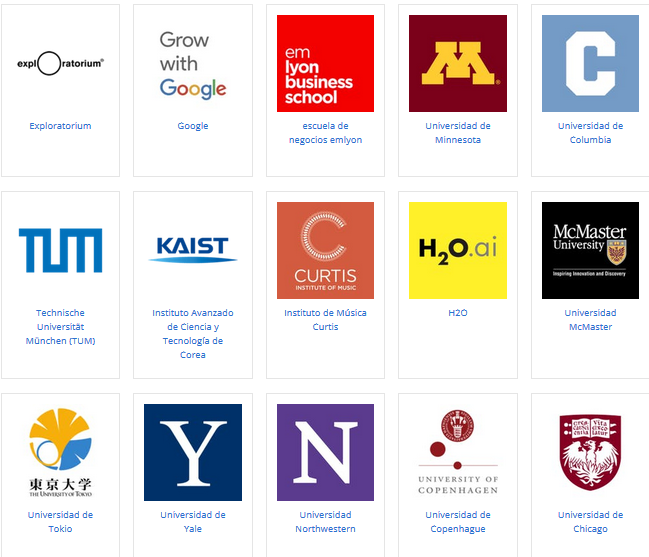
\includegraphics[width=12cm]{coursera10-3.png}
\caption{universidades e instituciones que forman parte de Coursera}
  \label{fig:cour10-3}
\end{figure}

\begin{figure}[H]
  \centering
	
\includegraphics[width=12cm]{coursera10-4.png}
\caption{universidades e instituciones que forman parte de Coursera}
  \label{fig:cour10-4}
\end{figure}

\begin{figure}[H]
  \centering
	
\includegraphics[width=12cm]{coursera10-5.png}
\caption{universidades e instituciones que forman parte de Coursera}
  \label{fig:cour10-5}
\end{figure}

\begin{figure}[H]
  \centering
	
\includegraphics[width=12cm]{coursera10-6.png}
\caption{universidades e instituciones que forman parte de Coursera}
  \label{fig:cour10-6}
\end{figure}

\begin{figure}[H]
  \centering
	
\includegraphics[width=12cm]{coursera10-7.png}
\caption{universidades e instituciones que forman parte de Coursera}
  \label{fig:cour10-7}
\end{figure}

\begin{figure}[H]
  \centering
	
\includegraphics[width=12cm]{coursera10-8.png}
\caption{universidades e instituciones que forman parte de Coursera}
  \label{fig:cour10-8}
\end{figure}

\begin{figure}[H]
  \centering
	
\includegraphics[width=11cm]{coursera10-9.png}
\caption{universidades e instituciones que forman parte de Coursera}
  \label{fig:cour10-9}
\end{figure}

\begin{figure}[H]
  \centering
	
\includegraphics[width=11cm]{coursera10-10.png}
\caption{universidades e instituciones que forman parte de Coursera}
  \label{fig:cour10-10}
\end{figure}

\section{Otras Plataformas de cursos MOOC}

Cada día aparecen nuevos proyectos informáticos, entre los cuales encontramos nuevas plataformas de cursos MOOC, muchas de ellas de pago. entre las que tenemos:

\begin{itemize}
\item Plataforma de cursos Platzi \footnote{https://platzi.com}.

\begin{figure}[H]
  \centering
	\includegraphics[width=11cm]{Platzi.png}
\caption{Plataforma de cursos MOOC, Platzi.}
  \label{fig:Platzi}
\end{figure}

\begin{itemize}
\item Plataforma de cursos Udemy \footnote{https://udemy.com}.

\begin{figure}[H]
  \centering
	\includegraphics[width=11cm]{Udemy.png}
\caption{Plataforma de cursos MOOC, Udemy.}
  \label{fig:Udemy}
\end{figure}

\item Plataformas de cursos BS Grupos \footnote{https://cursos.bsgrupo.com}.

\begin{figure}[H]
  \centering
	\includegraphics[width=11cm]{BSGInstitute.png}
\caption{Plataforma de cursos MOOC, BSGInstitute.}
  \label{fig:BSG}
\end{figure}

\item plataforma de cursos gratuitos en Ingles OM Personal \footnote{http://www.ompersonal.com.ar}.\

\begin{figure}[H]
  \centering
	\includegraphics[width=11cm]{OmPersonal.png}
\caption{Plataforma de cursos MOOC, OMPersonal.}
  \label{fig:OMP}
\end{figure}

\item Plataforma de cursos de pago en Ingles Open English \footnote{https://www.openenglish.com}.\

\begin{figure}[H]
  \centering
	\includegraphics[width=11cm]{Open-English.png}
\caption{Plataforma de cursos MOOC, Open English.}
  \label{fig:Open}
\end{figure}

\end{itemize}

\clearpage
\chapter{Google Académico}
Desde esta sección se inicia la búsqueda de información de calidad y validada\footnote{Los artículos científicos y libros previo a su publicación por parte de editoriales, pasan por procesos de revisión rigurosos por parte de evaluadores pares en el tema}, la cual se encuentra en forma de artículos científicos y libros, los cuales son resultados de procesos de investigación realizados por instituciones o personas particulares que a su vez han sido validadas previo a su publicación por pares académicos de editoriales especializadas, por lo tanto esta información es valida como \textbf{parte del estado del arte de una investigación.}

Para realizar búsquedas científicas, una de las primeras opciones que tenemos es ingresar a Google Académico\footnote{https://scholar.google.es/} y escribir en la barra de búsquedas el tema que estemos buscando.

\begin{figure}[ht]
  \centering
	\includegraphics[width=10cm]{google2.png}
\caption{Google Académico}
  \label{fig:google2}
\end{figure}

Por ejemplo, podemos realizar una búsqueda acerca de "\textbf{revisión sistemática}", la cual nos dará como resultados una serie de links, por lo general dirigidos a artículos científicos, tal como se muestra en la figura \ref{fig:google33}, muchos de los cuales pueden ser descargados y otros no. Los que \textbf{se pueden descargar de manera libre} son aquellos que tienen a la derecha un vinculo que puede comenzar con PDF O HTML y que con dar un clic sobre ellos nos dirigiremos al documento seleccionado. \\

\begin{figure}[ht]
  \centering
	\includegraphics[width=14cm]{google3.png}
\caption{Google Académico resultados de búsqueda}
  \label{fig:google33}
\end{figure}

Los \textbf{artículos científicos que no tienen ningún vinculo} a la derecha como podemos ver en la figura \ref{fig:google33}, \textbf{por lo general son de pago} y cuando damos un clic sobre ellos nos dirigiremos al sitio web de la revista en que ha sido publicado, en donde únicamente nos mostraran el resumen o Abstract, tal como se muestra en la figura \ref{fig:gogle55}.

\begin{figure}[ht]
  \centering
	\includegraphics[width=10cm]{google5.png}
\caption{Articulo Científico sin acceso}
  \label{fig:gogle55}
\end{figure}

Una ventaja que tenemos al leer el abstract es que nos dará una idea clara del contenido del articulo, lo cual te permitirá discernir entre seleccionarlo o descartarlo para tu \textbf{revisión sistemática} \footnote{El desarrollo de una revisión sistemática sera abordada en el capitulo, en el que se estudiara la herramienta Parsifal}, si el articulo nos interesa podemos tener acceso a el, previo al pago individual del mismo, o bien pagando una suscripción a la revista en que ha sido publicado\footnote{Si tiene problemas en esta parte, podemos asesorarlo, por favor escribanos a nuestra información de contacto}, lo cual nos permitirá ingresar a todas sus publicaciones o a las que determine nuestro contrato. En la figura \ref{fig:google4} nos muestra la parte inicial de un articulo, al cual si decides agregar a tu investigación, debes tomar sus datos de referencia por medio de un formulario de extracción de datos \footnote{Las referencias de artículos científicos sera abordada en el capitulo 6}. 

\begin{figure}[H]
  \centering
	\includegraphics[width=10cm]{google4.png}
\caption{Articulo Científico}
  \label{fig:google4}
\end{figure}

Ahora que conoces \textbf{Google Académico}, estas listo para iniciarte en el mundo de la investigación científica, leyendo artículos y libros en busca de información referente a tu tema de investigación, tienes que estar consciente para ello que el idioma universal del conocimiento es el Ingles, por lo que tu nivel debe ser al menos de comprensión lectora, si tienes problemas con el idioma, debes busca ayuda inscribiéndote en alguna academia local de idioma Ingles o tomar un curso en linea de pago o gratuitos.  como \textbf{OM Personal}\footnote{http://www.ompersonal.com.ar} 

\clearpage

\chapter{Gestores de Referencias Bibliográficas.}

Este capitulo te va a resultar muy interesante y clave para tu proyecto de investigación, ya que aprenderás a utilizar las herramientas online de gestión bibliográfica, Mendeley y Zotero, de acuerdo a tus preferencias una de ellas o ambos,  se convertirán en una de las herramientas mas importantes e imprescindible en tu proceso diario de investigación. Un gestor de referencias bibliográficas permite crear, almacenar, organizar, compartir e insertar referencias bibliográficas, en procesadores de textos existes, tales como Microsoft Word y las diferentes versiones latex. Lo mejor de estos gestores bibliográficos es que podrás disponer de tu base de datos de referencias cuando las necesites con solo acceder a las versiones en linea y utilizarlas en la plataforma de tu preferencia.  

\section{Mendeley}

Mendeley es una aplicación Web y de escritorio desarrollado por Elsevier \cite{ElsevierElsevierKnowledge}, tiene versiones gratuitas y de pago, los cuales se sincronizan entre si, sus principales características son:

\begin{itemize}
\item Gestionar y compartir referencias bibliográficas.
\item Gestionar y compartir documentos de investigación.
\item Encontrar nuevas referencias y documentos.
\item Trabajo colaborativo en linea.
\end{itemize}

Para comenzar a trabajar con \textbf{Mendeley}, debes escribir en el navegador(Web browser) de tu computador, tablet o Smart Phone, su dirección electrónica \footnote{https://www.mendeley.com},
e inmediatamente veras cargar su pagina principal tal como se muestra en la figura \ref{fig:mendeley1}.

Si miras en la parte superior derecha de la pantalla, podrás observar tres iconos:

\begin{itemize}
\item \textbf{Sign in.} El cual nos permite acceder a Mendeley on line, si estamos registrados en la aplicación.
\item \textbf{Create Account.} El cual nos permite crear una cuenta en Mendeley. 
\item \textbf{Download.} El cual nos permite realizar descarga de aplicativos de Mendeley.
\end{itemize}

\begin{figure}[ht]
  \centering
	\includegraphics[width=10cm]{mendeley1.png}
\caption{Pagina Principal de Mendeley}
  \label{fig:mendeley1}
\end{figure}

Ahora llego el momento de que configures tu computador, para poder comenzar a adicionar referencias de artículos científicos, libros u cualquier otro documento, directamente desde tu navegador web, para ello accedemos al icono \textbf{download}, desde el cual podemos realizar las siguientes descargas:  

\begin{itemize}
\item \textbf{Mendeley desktop.} Esta opción permite descargar el aplicativo de escritorio tal como se muestra en la figura \ref{fig:mendeley2}, con el cual puedes gestionar tu bibliografía sin necesidad de estar conectado al internet. Medeley desktop se sincroniza con tu aplicación con Mendele online, para realizar tus actualización  bibliográficas, este aplicativo esta disponible para equipos con sistemas operativos Windows, Mac OS y Linux.

\begin{figure}[ht]
  \centering
	\includegraphics[width=10cm]{mendeley2.png}
\caption{Mendeley desktop}
  \label{fig:mendeley2}
\end{figure}

Una vez descargado e instalado el aplicativo en el escritorio de tu computador, se vera de como vemos en la figura \ref{fig:mendeley3}. 

\begin{figure}[H]
  \centering
	\includegraphics[width=10cm]{mendeley3.png}
\caption{Mendeley desktop}
  \label{fig:mendeley3}
\end{figure}

 Ahora te queda únicamente explorar el aplicativo, el cual esta dividido en cinco  secciones:

\begin{enumerate}
\item \textbf{Menú e iconos de la barra superior.} Aquí podrás ver la pantalla principal de Mendeley Desktop, tal como muestra la figura \ref{fig:mendeley3}, la cual en su parte superior contiene un  menú de opciones, que muestra la figura \ref{fig:mendeley4}, el cual contiene las siguientes opciones: file, edit, tools y help, luego una serie de iconos y finalmente la barra de búsqueda de artículos. 

\begin{figure}[H]
  \centering
	\includegraphics[width=5cm]{mendeley4.png}
\caption{Menú de Opciones Mendeley}
  \label{fig:mendeley4}
\end{figure}

El icono \textbf{Sincronización}, que muestra la figura \ref{fig:mendeley5} permite sincronizar o actualizar la información de las referencias bibliográficas de Mendeley Desktop desde Mendeley web, ya que allí se guardan las referencias bibliográficas que  realizas o capturas.  

\begin{figure}[H]
  \centering
	\includegraphics[width=2cm]{mendeley5.png}
\caption{Sincronización}
  \label{fig:mendeley5}
\end{figure}

\item \textbf{Área de control.} En esta área del aplicativo podrás entre otras opciones tal como muestra la figura \ref{fig:mendeley6}, \textbf{crear carpetas} y \textbf{crear grupos}.

\begin{figure}[H]
  \centering
	\includegraphics[width=4cm]{mendeley6.png}
\caption{Área de control}
  \label{fig:mendeley6}
\end{figure}

\item \textbf{Filtro por autor.} En esta opción podrás filtrar el contenido de tus referencias por autor, simplemente con seleccionarlo, tal como muestra la figura \ref{fig:mendeley7}, lo que nos permite dar incluso los metadatos de la referencia seleccionada.

\begin{figure}[H]
  \centering
	\includegraphics[width=12cm]{mendeley7.png}
\caption{Filtro por autor}
  \label{fig:mendeley7}
\end{figure}

\item \textbf{Documentos.} En esta parte de la aplicación, puedes observar todas las referencias que has capturado, para la realización de cada uno de tus proyecto, tal como se muestra en la figura \ref{fig:mendeley8}.

\begin{figure}[H]
  \centering
	\includegraphics[width=10cm]{mendeley8.png}
\caption{Documentos}
  \label{fig:mendeley8}
\end{figure}

\item \textbf{Detalle de artículos.} En esta parte de la aplicación, podemos observar los metadatos del articulo seleccionado, tal como se muestra en la figura \ref{fig:mendeley9}.

\begin{figure}[H]
  \centering
	\includegraphics[width=5cm]{mendeley9.png}
\caption{Detalle de artículos}
  \label{fig:mendeley9}
\end{figure}

\end{enumerate}

\item \textbf{Web Importer.} Este aplicativo una vez descargado y configurado en tu navegador web, te permitirá capturar los metadatos de los artículos científicos, libros u cualquier otro documento, que desees directamente a tu librería en Mendeley online, tal como vemos en la figura \ref{fig:mendeley10}, cabe indicar que en esta parte puedes guardar tus diferentes proyectos en carpetas individuales.

\begin{figure}[H]
  \centering
	\includegraphics[width=5cm]{mendeley10.png}
\caption{Navegadores + Web Importer}
  \label{fig:mendeley10}
\end{figure}

Para configurar Web Importer, debes seleccionar el navegador de tu preferencia y a continuación descargar el aplicativo en el navegador web. tal como se muestra en la figura \ref{fig:mendeley11} 

\begin{figure}[H]
  \centering
	\includegraphics[width=5cm]{mendeley11.png}
\caption{Web Importer}
  \label{fig:mendeley11}
\end{figure}

Para finalmente poderlo tener en forma de icono en nuestro navegador web, tal como vemos en la figura \ref{fig:mendeley12}. 

\begin{figure}[H]
  \centering
	\includegraphics[width=2cm]{mendeley12.png}
\caption{Icono de Web importer}
  \label{fig:mendeley12}
\end{figure}


\item \textbf{Citation Plugin.} Con este plugin puedes administrar tus referencias bibliográficas y organizar tu investigación en Microsoft Word Mac o Libre Office (todas las plataformas), tal como vemos en las figura \ref{fig:mendeley13}. Una vez configurado tu procesador de texto favorito, podrás a la vez de comenzar a escribir un articulo, libro o cualquier otro documento,  insertar de forma rápida y sencilla citas con estilo para materiales de referencia de tu Biblioteca de Mendeley.

\begin{figure}[H]
  \centering
	\includegraphics[width=6cm]{mendeley13.png}
\caption{Citation Plugin}
  \label{fig:mendeley13}
\end{figure}

Generar automáticamente una bibliografía para tu trabajo con todos los materiales que has citado, elegir entre una enorme y creciente biblioteca de estilos de citas y actualizar fácilmente todas las citas con unos pocos clics.

\end{itemize}

Una vez que ya tienes una cuenta de mendeley, configurado Mendeley desktop, Citation Plugin y el navegador web de tu computador, estas listo para comenzar a realizar el trabajo de adicionar a tu librería mendeley las referencias de metadatos de los documentos a utilizar en tu proyecto de investigación. A continuación detallamos la forma en que puedes capturar la información de cada uno tus artículos:

\begin{enumerate}
    \item Inicialmente debes cargar el articulo o documento del cual quieras adicionar sus metadatos, a tu  base de datos de referencia bibliográfica, tal como podemos observar en la figura  \ref{fig:mendeley14}.
    
    \begin{figure}[H]
    \centering
	\includegraphics[width=8cm]{mendeley14.png}
    \caption{Articulo científico}
    \label{fig:mendeley14}
    \end{figure}
    
    \item Debes seleccionar en tu navegador web el icono de \textbf{web importer}, tal como vemos en la figura \ref{fig:mendeley15}.  
    
    \begin{figure}[H]
    \centering
	\includegraphics[width=2cm]{mendeley12.png}
    \caption{Icono de Web importer}
    \label{fig:mendeley15}
    \end{figure}

    \item En la figura \ref{fig:mendeley16}, te muestra el documento con la ventana de captura automático de datos de mendeley, en esta parte hay que cerciorarse que los datos tomados estés completos, o caso contrario debes ingresarlos de manera manual, para que la bibliografía que contenga tu documento este completa para a continuación seleccionar \textbf{save}.
    
    \begin{figure}[H]
    \centering
	\includegraphics[width=8cm]{mendeley15.png}
    \caption{Articulo + Web importer}
    \label{fig:mendeley16}
    \end{figure}

    \item Ahora puedes cerciorarte que las referencias de tus artículos se guardaron correctamente en tu base bibliográfica de Mendeley, para ello en la parte superior de la ventana de captura de datos de mendeley que viste en la figura \ref{fig:mendeley17} das clic en su parte superior en la opción \textbf{Web library}, la cual automáticamente te lleva a tu cuenta en el sitio web de mendeley, tal como se puede ver en la figura \ref{fig:mendeley16}.
    
    \begin{figure}[H]
    \centering
	\includegraphics[width=8cm]{mendeley16.png}
    \caption{Cuenta de sitio web de Mendeley}
    \label{fig:mendeley17}
    \end{figure}
    
    \item El siguiente paso en que abras tu mendeley de escritorio y sincronices sus datos con los de tu cuenta web, tal como se puede ver en la figura \ref{fig:mendeley18} y \ref{fig:mendeley19}.
    
    \begin{figure}[H]
    \centering
	\includegraphics[width=10cm]{mendeley3.png}
    \caption{Mendeley desktop}
    \label{fig:mendeley18}
    \end{figure}

    \begin{figure}[H]
    \centering
	\includegraphics[width=2cm]{mendeley5.png}
    \caption{Sincronización}
    \label{fig:mendeley19}
    \end{figure}
\end{enumerate}

\section{Trabajar en Microsoft Word con Mendeley}

En esta sección te explicaremos como poder trabajar con el gestor de referencias bibliográficas Mendeley en Microsoft Word, para ello debes configurar el plugin de mendeley en el procesador de textos, siguiendo los siguientes pasos.

\begin{enumerate}
    \item El primer paso es tener instalado \textbf{Mendeley Desktop}
    \item Abrir Microsoft Word y verificar si en la opción de referencias aparece el icono de Mendeley, si aparece podemos comenzar a escribir e insertar referencias en nuestro documento.
    \item Si no aparece el icono de Mendeley en Word, tendrás que ir a Mendeley de escritorio y en el menú tools, seleccionar la opción \textbf{Install Ms Word Plugin}, tal como lo vemos en la figura \ref{fig:mendeley20}, si no se activa el icono en Word, deberás hacer clic en \textbf{Uninstall Ms Word Plugin}, no necesitamos instalarlos y debemos verificar en Microsoft Word si el icono de mendeley aparece en la opción de referencias.
    
    \begin{figure}[H]
    \centering
	\includegraphics[width=8cm]{mendeley17.png}
    \caption{Mendeley Desktop}
    \label{fig:mendeley20}
    \end{figure}
    
    \item Si aún no esta activada Mendeley, debemos abrir Microsoft Word y realizar los siguientes pasos:
    
    \begin{itemize}
        \item Seleccionar en la barra de Menú \textbf{Archivo}
        \item A continuación seleccionar \textbf{Opciones}, la cual te llevara a la ventana \textbf{Opciones}, en el cual debemos escoger la opción \textbf{Complementos} tal como vez en la figura \ref{fig:mendeley21}, en la cual deberás buscar en el área de complementos \textbf{Mendeley} y dar aceptar, generalmente esto debe activar el complemento.

        \begin{figure}[H]
        \centering
    	\includegraphics[width=10cm]{mendeley18.png}
        \caption{Ventana Opciones}
        \label{fig:mendeley21}
        \end{figure}
        
        \item Si aún no esta activo el complemento, debes ir a la parte inferior de la ventana y en la barra \textbf{Administrar} seleccionar \textbf{Complementos de Word} y hacer clic en \textbf{Ir}, tal como ves en la figura \ref{fig:mendeley22}.
        
        \begin{figure}[H]
        \centering
    	\includegraphics[width=8cm]{mendeley19.png}
        \caption{Ventana opciones}
        \label{fig:mendeley22}
        \end{figure}
        
        \item Inmediatamente se abrirá la ventana \textbf{Plantilla y complementos}, tal como ves en la figura \ref{fig:mendeley23}, se debe escoger el icono \textbf{Agregar} y seleccionar Mendeley y aceptar. 
        
        \begin{figure}[H]
        \centering
    	\includegraphics[width=8cm]{mendeley20.png}
        \caption{Plantilla y complementos}
        \label{fig:mendeley23}
        \end{figure}
        
        \item Si no aparece el complemento de mendeley debes buscarlo por lo general en la siguiente dirección "Program Files (x86)\Mendeley Desktop\wordPlugin", tal como ves en la figura \ref{fig:mendeley24}

        \begin{figure}[H]
        \centering
    	\includegraphics[width=8cm]{mendeley21.png}
        \caption{Ruta de archivo Mendeley}
        \label{fig:mendeley24}
        \end{figure}

        \item A continuación seleccionamos el plugin y das aceptar, como ves en la figura \ref{fig:mendeley25}
        
        \begin{figure}[H]
        \centering
    	\includegraphics[width=8cm]{mendeley22.png}
        \caption{Plantillas y complementos}
        \label{fig:mendeley25}
        \end{figure}

        \item Finalmente podremos ver como se activa el icono de mendely en la ventana de \textbf{referencias} de \textbf{Microsft word}, tal como ves en la figura \ref{fig:mendeley26}.
        
        \begin{figure}[H]
        \centering
    	\includegraphics[width=8cm]{mendeley23.png}
        \caption{Ventana opciones}
        \label{fig:mendeley26}
        \end{figure}
      
    \end{itemize}
\end{enumerate}

Una vez que ya tenemos el icono de Mendeley en la ventana de \textbf{referencias} de \textbf{Microsoft Word}, puedes comenzar a trabajar en tu proyecto con las referencias que hayas anexado a tu base de datos bibliográfica Mendeley, con solo ubicarnos en la parte del texto que deseemos y presionar el icono \textbf{Insertar Cita o Insert Citation}, figura \ref{fig:mendeley27}.

        \begin{figure}[H]
        \centering
    	\includegraphics[width=8cm]{mendeley24.png}
        \caption{Insertar Cita}
        \label{fig:mendeley27}
        \end{figure}

En el siguiente ejemplo veras como una vez que estas ubicado, en la parte del documento en que deseas insertar una cita y das clic en el icono \textbf{Insertar Cita o Insert Citation},  aparece una ventana en la cual puedes en su barra de búsqueda, buscar y seleccionar el articulo que necesites, como lo ves en la figura \ref{fig:mendeley28}.

        \begin{figure}[H]
        \centering
    	\includegraphics[width=8cm]{mendeley25.png}
        \caption{Insertar Citas en Word}
        \label{fig:mendeley28}
        \end{figure}

Finalmente una vez que ya has anexado a tu documento las citas bibliográficas necesarias, deberás escoger en el menú la opción \textbf{Referencias}, y dar clic en el icono \textbf{Insert Bibliography}, para insertar al final del documento la bibliografía utilizada, tal como lo ves en la figura \ref{fig:mendeley29}.

        \begin{figure}[H]
        \centering
    	\includegraphics[width=8cm]{mendeley26.png}
        \caption{Insertar Citas en Word}
        \label{fig:mendeley29}
        \end{figure}

Cabe indicar que las referencias pueden ser importadas y exportadas de mendeley por medio de archivos .bib, con los cuales se puede trabajar en otros aplicativos como por ejemplo \textbf{overleaf}, el cual es un látex online, el cual también se estudiara en este libro.

\clearpage

\section{Zotero}

\chapter{Bases de datos científicas o bibliográficas}\label{sec:basesdedatos}

Las bases de datos científicas o bibliográficas, son una recopilación de documentos de índole científico, entre los cuales tenemos: 

\begin{itemize}
\item Artículos de revistas científicas
\item Libros
\item Congresos
\item Etc.
\end{itemize}

Cabe indicar que para poder acceder al contenido de las bases de datos, hay que pagar una subscripción de manera personal, o mediante una subscripción de la entidad académica a la cual perteneces, cabe indicar que la mayor parte de investigadores, docentes y estudiantes se acogen a esta opción. En caso de que la institución académica a la que perteneces no esta suscrita a la base de datos de tu interés, te sugerimos envíes una carta a las autoridades respectivas, para que se suscriban a la misma y puedas continuar con tu investigación. A continuación podrás ver los logos de acceso de un grupo de bases de datos, a las cuales por lo general se acceden desde las paginas web de las universidades o entidades de investigación:

        \begin{figure}[H]
        \centering
    	\includegraphics[width=10cm]{basesdedatos1.png}
        \caption{Bases de datos de Conocimiento}
        \label{fig:basededatos1}
        \end{figure}

        \begin{figure}[H]
        \centering
    	\includegraphics[width=10cm]{basesdedatos2.png}
        \caption{Bases de datos de Conocimiento}
        \label{fig:basededatos2}
        \end{figure}

        \begin{figure}[H]
        \centering
    	\includegraphics[width=10cm]{basesdedatos3.png}
        \caption{Bases de datos de Conocimiento}
        \label{fig:basededatos3}
        \end{figure}

        \begin{figure}[H]
        \centering
    	\includegraphics[width=10cm]{basesdedatos4.png}
        \caption{Bases de datos de Conocimiento}
        \label{fig:basededatos4}
        \end{figure}


Ahora que ya conoces al menos el nombre de un grupo de las principales bases de datos científicas del mundo, debes aprender a realizar la búsqueda de información en una base de datos, tomando en cuenta que este tipo de búsqueda son muchas mas complejas y detalladas que una búsqueda en google o cualquier otro motor de búsqueda a ese nivel, tienes que estar totalmente seguro de la temática a consultar, puesto que la base de datos nos dará los resultados de acuerdo a como nosotros la consultemos. Para tener una mayor comprensión de la forma de como preguntar de manera correcta a la base de datos respecto a un tema, existe una técnica llamada PICO, la cual se basa en evidencia, su estructura la podemos ver en la tabla \ref{tbl:pico}:

\begin{table}[H]
\centering
\footnotesize
\begin{tabular}{|l|l|l|}
\hline
$\enspace$ \textbf{P} & Población & Población a investigar \\  
\hline
$\enspace$ \textbf{I} & Intervención & Que vamos a investigar \\  
\hline
$\enspace$ \textbf{C} & Comparación & Como vamos a comparar la información \\  
\hline
$\enspace$ \textbf{O} & Resultado & Resultados alcanzados\\  
\hline
\end{tabular}
\caption{Método PICO}
\label{tbl:pico}
\end{table} 

Cabe indicar que a partir del Método PICO, podrás obtener lo que se conoce como cadena de búsqueda, la cual es la forma en que se realiza búsquedas de información en las bases de datos. Un ejemplo de una cadena de búsqueda es:

(ALL("Natural Language Processing") AND ALL(suicidal AND prevention) OR ALL(suicidal AND ideation)) AND PUBYEAR > 2016 

En este libro aprenderás a trabajar con tres de las principales bases de datos  académicas \textbf{Scopus, Web of Science e IEEE}, a las que accederás de dos formas, por medio de una cuenta personal o una institucional, por ello te recomendamos que accedas a un manual de acceso que debe ser proporcionado por la institución educativa a la que perteneces.

\clearpage
\subsection{Scopus}

Scopus, es una base de datos bibliográficos de resúmenes y citas de literatura revisada por pares que abarca entre otras áreas del conocimiento \textbf{ciencia, tecnología, medicina, ciencia sociales, arte y humanidades}, esto permite a los  usuarios descubrir y analizar el mundo de la investigación. Scopus cuenta con tres métricas de factor de impacto de la investigación como son \textbf{Scimago Journal Rank (SJR)\footnote{https://www.scimagojr.com/}, SNIP (Source-normalized impact Paper)\footnote{http://www.journalindicators.com/} y CiteScore\footnote{https://www-scopus-com.consultaremota.upb.edu.co/sources}}. Los tipos de documentos que publican las revistas científicas que pertenecen a Scopus son: artículos científicos, revisiones, articulos de conferencias libros y actas de conferencias.

       \begin{figure}[H]
        \centering
    	\includegraphics[width=12cm]{Scop1.png}
        \caption{Scopus}
        \label{fig:scop1}
        \end{figure}

La pagina web de Scopus\footnote{http://www.scopus.com}, tal como se muestra en la figura \ref{fig:scop2}, permite realizar diferentes tipos de búsqueda.  
 
        \begin{figure}[H]
        \centering
    	\includegraphics[width=12cm]{Scop2.png}
        \caption{Scopus}
        \label{fig:scop2}
        \end{figure}

Previo a realizar una búsqueda correcta de bibliografía, se debe tener ya un conocimiento
aunque sea básico del tema a investigar y contar con una lista de palabras claves del
mismo, con estas se debe generar una cadena de búsqueda, tal como ya se a explicado previamente. Los diferentes
tipos de búsquedas de Scopus son:

\begin{itemize}
    \item \textbf{Documents}

 La opción búsqueda por \textbf{Documentos}, tal como se ve en la figura \ref{fig:scop3}, muestra en la linea de búsqueda la palabra \textbf{Search}, en la cual se debe ingresar la palabra o silaba a buscar, para a continuación seleccionar el tipo de campo del documento por el cual buscaremos, \textbf{All fields; Article title, abstract, keywords; authors; First author; Source title; Article title; Abstract; Keywords; Affiliation (Affiliation name, Affiliation city, Affiliation country); Funding information (Funding sponsor, Funding acronym, Funding number); Language; ISSN; CODEN; DOI; References; Conference; Article title; Abstract, Keywords, Authors; Chemical name; CAS number; ORCID}. 
 

        \begin{figure}[H]
        \centering
    	\includegraphics[width=12cm]{Scop3.png}
        \caption{Búsqueda por Documentos}
        \label{fig:scop3}
        \end{figure}

Seguidamente, si necesitamos adicionar una nueva palabra o silaba para complementar la búsqueda, se debe dar clic sobre el icono \textbf{+}, acción que incrementara una nueva linea de búsqueda, previo a escoger el operador lógico requerido \textbf{OR, AND y NOT}. Finalmente una vez que ya este lista la secuencia de búsqueda, se debe dar clic en el icono \textbf{Search}, para que la plataforma realice la búsqueda. 

    \item \textbf{Authors}

La búsqueda por \textbf{author} que vemos en la figura \ref{fig:scop4}, es muy útil, ya que permite realizar búsquedas por \textbf{Autor, afiliación o código ORCID\footnote{https://orcid.org/}}, de manera individual o combinándolas entre si.

        \begin{figure}[H]
        \centering
    	\includegraphics[width=12cm]{Scop4.png}
        \caption{Búsqueda por Autores}
        \label{fig:scop4}
        \end{figure}
        
Al buscar por \textbf{Author}, debemos escribir sus nombres en los campos \textbf{Author last name (Apellido)} y  
\textbf{Author first name(Nombre)}, y a continuación dar clic en el icono \textbf{Search}, para iniciar la búsqueda. tal como vemos en la figura \ref{fig:scop5}.  

        \begin{figure}[H]
        \centering
    	\includegraphics[width=12cm]{Scop5.png}
        \caption{Búsqueda por Autores}
        \label{fig:scop5}
        \end{figure}

Seguidamente podemos ver los resultados, tal como muestra la imagen \ref{fig:scop6}, en la cual se puede ver datos de las publicaciones del autor, tales como: \textbf{Numero de documentos publicados, institución con la cual publica, ciudad y país}.

        \begin{figure}[H]
        \centering
    	\includegraphics[width=12cm]{Scop6.png}
        \caption{Búsqueda por Autores}
        \label{fig:scop6}
        \end{figure}

Al buscar por \textbf{Affiliation}, debemos escribir el nombre de la institución por la cual queremos buscar y a continuación dar clic en el icono \textbf{Search}, para iniciar la búsqueda. tal como vemos en la figura \ref{fig:scop7}.  

        \begin{figure}[H]
        \centering
    	\includegraphics[width=12cm]{Scop7.png}
        \caption{Búsqueda por Autores}
        \label{fig:scop7}
        \end{figure}

Tal como muestra la imagen \ref{fig:scop8}, se puede ver datos los datos de la institución buscada, tales como: \textbf{Affiliation name, affiliation, institution, city, country}.

        \begin{figure}[H]
        \centering
    	\includegraphics[width=12cm]{Scop8.png}
        \caption{Búsqueda por Autores}
        \label{fig:scop8}
        \end{figure}

Cuando se desea realizar una búsqueda por autor, se tiene además la opción de realizar la búsqueda por medio del código \textbf{ORCID}, el cual es una afiliación global de investigadores, para ello se debe escribir el código ORCID del autor y a continuación dar clic en el icono \textbf{Search}, para iniciar la búsqueda. tal como vemos en la figura \ref{fig:scop9}.  

        \begin{figure}[H]
        \centering
    	\includegraphics[width=12cm]{Scop9.png}
        \caption{Búsqueda por Autores}
        \label{fig:scop9}
        \end{figure}

A continuación aparecerán si el autor tiene publicaciones en Scopus, un listado de estas, caso contrario la pagina nos dirá que no encontró las publicaciones.
    
    \item \textbf{Affiliations}
    
Por medio de la opción \textbf{Affiliations}, se puede encontrar a institución registrada en Scopus, tal como vemos en la imagen \ref{fig:scop10}. Esta opción distingue el Identificador entre afiliaciones.   

        \begin{figure}[H]
        \centering
        \includegraphics[width=12cm]{Scop10.png}
        \caption{Búsqueda por Affiliations}
        \label{fig:scop10}
        \end{figure}    

Al asignar a cada afiliación en Scopus un número único y agrupar todos los documentos afiliados a una organización, tal como lo vemos en la figura \ref{fig:scop11}. 

         \begin{figure}[H]
        \centering
        \includegraphics[width=12cm]{Scop11.png}
        \caption{Búsqueda por Affiliations}
        \label{fig:scop11}
        \end{figure}    

Entre la información que se despliega por cada institución encontramos: \textbf{Affiliation name, affiliation, institution, city, country}, los cuales al dar clic sobre ellos nos muestra información de utilidad:

\textbf{Affiliation name}, al dar clic sobre el nombre de la institución inmediatamente se despliega  la figura \ref{fig:scop12}, la cual muestra estadísticas en cuento a publicaciones realizadas por individuos adscritos a la institución.

         \begin{figure}[H]
        \centering
        \includegraphics[width=12cm]{Scop12.png}
        \caption{Búsqueda por Affiliations}
        \label{fig:scop12}
        \end{figure}    

\textbf{Affiliation} , al dar clic sobre el numero de afiliación de la institución inmediatamente se despliega la figura \ref{fig:scop13}, la cual busca el numero de publicaciones realizadas por individuos adscritos a la institución y las despliega. Hay que tener en cuenta que al dar clic sobe \textbf{institution}, nos daran los mismos resultados que muestra la figura \ref{fig:scop13}.

        \begin{figure}[H]
        \centering
        \includegraphics[width=12cm]{Scop13.png}
        \caption{Búsqueda por Affiliations}
        \label{fig:scop13}
        \end{figure}    
    
    \item \textbf{Advanced}
    
La opción \textbf{Advanced}, es para usuarios con algo de experiencias en la búsqueda de información y en la realización de cadenas de búsqueda, tal como vemos en la figura \ref{fig:scop14}, se introduce una primera cadena con las palabras o silabas claves de nuestra proyecto de investigación y a continuación damos un clic en el icono \textbf{Search}, para iniciar la búsqueda.

        \begin{figure}[H]
        \centering
        \includegraphics[width=12cm]{Scop14.png}
        \caption{Búsqueda Advanced}
        \label{fig:scop14}
        \end{figure}    

\end{itemize}

Una vez realizado el proceso de búsqueda, por medio de la cadena de palabras claves, podemos observar los resultados de la misma, tal como se muestra en la figura \ref{fig:scop15}, la cual permite ver documentos relacionados con nuestro tema de investigación para su lectura y posterior inclusión o exclusión de nuestra investigación.

        \begin{figure}[H]
        \centering
    	\includegraphics[width=10cm]{Scop15.png}
        \caption{Scopus}
        \label{fig:scop15}
        \end{figure}

La búsqueda realizada, a su vez puede ser mejorada si se refina la misma, seleccionando entre las diferentes opciones que Scopus permite para esta función, lmismas que se se ven en la figura \ref{fig:Scop16}, para a continuación una vez seleccionadas, hacer clic en el icono \textbf{Limit To} or \textbf{Exclude}, de acuerdo a nuestro requerimientos.


        \begin{figure}[H]
        \centering
        \includegraphics[width=12cm]{Scop16.png}
        \caption{Refine results}
        \label{fig:Scop16}
        \end{figure}    

Finalmente una vez que nuestra búsqueda de documentos en Scopus este completa, debemos seleccionarlos y marcarlos, para así poder exportarlos a otras aplicaciones, para ello debemos escoger el casillero seleccionar resultados de pagina y escoger el numero de resultados que queremos ver, figura \ref{fig:scop17}, siendo el numero máximo 200, su vez una vez que se visualicen estos deben ser marcados de forma general dando clic en el casillero \textbf{All}, o marcándolos de manera individual, para a continuación dar clic en el icono \textbf{Add to List}, para agregarlos a tu lista temporal.

        \begin{figure}[H]
        \centering
    	\includegraphics[width=10cm]{Scop17.png}
        \caption{results per page}
        \label{fig:scop17}
        \end{figure}

En la figura \ref{fig:scop18}, podemos ver el numero de elementos agregados a nuestra lista temporal. 

        \begin{figure}[H]
        \centering
    	\includegraphics[width=10cm]{Scop18.png}
        \caption{Add to list}
        \label{fig:scop18}
        \end{figure}

Seguidamente mientras este seleccionada la opción \textbf{All}, podemos dar clic en la opción \textbf{Export}, para exportar los metadatos de los documentos por medio de uno de los tipos de archivos que Scopus permite, tal como vemos en la figura \ref{fig:scop19}. Los tipos de archivos en los que se puede exportar los documentos son: \textbf{Mendeley; RefWorks; RIS Format, EndNote, Reference Manager; CSV Excel; BibTeX; Plain Text, ASCII in HTML}. 


     \begin{figure}[H]
        \centering
    	\includegraphics[width=10cm]{Scop19.png}
        \caption{Configuración de exportación de documentos}
        \label{fig:scop19}
        \end{figure}

En la figura \ref{fig:scop20}, se puede ver marcadas los datos de los documentos que se van a exportar, asi como el tipo de archivo seleccionado, en este caso \textbf{BibTeX}, finalmente se selecciona el icono \textbf{Export}, para que se inicie la descarga del archivo con el formato escogido.

     \begin{figure}[H]
        \centering
    	\includegraphics[width=10cm]{Scop20.png}
        \caption{Configuración de exportación de documentos}
        \label{fig:scop20}
        \end{figure}

Posterior a dar clic en exportar, aparece la imagen \ref{fig:scop21}, en la cual podremos escoger abrir el documento o descargarlo.

     \begin{figure}[H]
        \centering
    	\includegraphics[width=6cm]{Scop21.png}
        \caption{Configuración de exportación de documentos}
        \label{fig:scop21}
        \end{figure}

La Opción \textbf{Analyze search results}, es de gran utilidad para el investigador, ya que permite a partir de los documentos encontrados, por medio de la cadena de búsqueda, obtener diferentes datos estadísticos, los cuales se pueden agregar a la investigación. 

        \begin{figure}[H]
        \centering
    	\includegraphics[width=6cm]{Scop22.png}
        \caption{Analyze search results}
        \label{fig:scop22}
        \end{figure}

En las figura \ref{fig:scop23} se puede apreciar los años en que fueron publicados los articulos encontrados y en el figura \ref{fig:scop24}, podemos observar una serie de estadísticas del conjunto de nuestros documentos. Las estadísticas que proporciona Scopus son: \textbf{Documents per year by source; Documents by author; Documents by affiliation; Documents by country/territory; Documents by type; Documents by subject area; Documents by funding sponsor}.

        \begin{figure}[H]
        \centering
    	\includegraphics[width=12cm]{Scop23.png}
        \caption{Analyze search results}
        \label{fig:scop23}
        \end{figure}

Cabe indicar que si damos clic sobre cualquiera de los elementos de la figura \ref{fig:scop24}, obtendremos una nueva pantalla con mayor cantidad de datos sobre el tema.

        \begin{figure}[H]
        \centering
    	\includegraphics[width=12cm]{Scop24.png}
        \caption{Analyze search results}
        \label{fig:scop24}
        \end{figure}




\clearpage
\subsection{Web of Science}

Web of Science (WOS)\footnote{https://clarivate.com/products/web-of-science/}, al igual que Scopus es una de las principales bases de datos bibliográficas de citas de artículos científicos, libros y otro tipo de documento, suministrados por Thomson Reuters, propiedad de Clarivate Analytics. La figura \ref{fig:WOS1} muestra la pagina de inicio de WoS, desde esta pagina si poses una clave de acceso (Por lo general institucional) puedes acceder a la pagina de búsqueda de información.

        \begin{figure}[H]
        \centering
    	\includegraphics[width=10cm]{Wos1.png}
        \caption{Pagina principal de Web of Science}
        \label{fig:WOS1}
        \end{figure}

La pagina de búsqueda de WoS, tal como se muestra en la figura \ref{fig:WOS2}, permite realizar diferentes tipos de búsqueda. 

        \begin{figure}[H]
        \centering
    	\includegraphics[width=10cm]{Wos2.png}
        \caption{Búsquedas de Documentos}
        \label{fig:WOS2}
        \end{figure}

Al igual como se menciono anteriormente(Scopus), para realizar una búsqueda correcta de bibliografía es necesario un conocimiento aunque sea básico del tema a investigar y contar con una lista de palabras claves del mismo, para generar la cadena de búsqueda. 
Los diferentes tipos de búsquedas de WoS son:

\begin{itemize}
\item \textbf{Búsqueda básica}

Para realizar la \textbf{Búsqueda básica} tal como se ve en la figura \ref{fig:WOS3}, debemos ingresar en el casillero de búsqueda nuestra palabra o frase clave, a continuación seleccionar el item de busque entre \textbf{Tema, titulo, autor, nombre de publicación, año de publicación, entidad financiadora, prefOrganización-Consolidada, todos los campos, número de acceso, dirección, identificadores de autores, conferencia, tipo de documentos, DOI, editor, número de concesión, autoría conjunta, idioma, ID de PubMed}, a continuación si se necesita se puede agregar una fila para añadir a la búsqueda una nueva palabra clave anteponiendo el operador lógico \textbf{And, Or o Not}, según sea el tema, para finalmente escoger el icono buscar. 

    \begin{figure}[H]
    \centering
    \includegraphics[width=10cm]{Wos3.png}
    \caption{Búsqueda básica}
    \label{fig:WOS3}
    \end{figure}

\item \textbf{Búsqueda de referencia citada}

La \textbf{Búsqueda de referencia citada}, la cual vemos en la figura \ref{fig:WOS4}, es de gran ayuda por cuanto personaliza búsquedas por ítems como \textbf{Autor citado, trabajo citado, DOI citado, año(s) de cita, volumen citado, número citado, páginas citadas, título citado}. Es muy interesante para búsquedas individuales, pero no funciona como cadena de búsqueda general.

    \begin{figure}[H]
    \centering
    \includegraphics[width=10cm]{Wos4.png}
    \caption{Búsqueda de referencia citada}
    \label{fig:WOS4}
    \end{figure}


\item \textbf{Búsqueda avanzada}

La \textbf{Búsqueda avanzada}, la cual vemos en la figura \ref{fig:WOS4} requiere algo mas de experiencia por parte del investigador, en esta el mismo debe escribir directamente en el casillero su cadena de búsqueda, ingresando las palabras claves de su investigación, con sus respectivos operadores lógicos, y comenzar a probar los resultados de la búsqueda, si el numero de documentos es muy alto deberá comenzar a limitar la misma por medio de los ítems \textbf{Tema, titulo, autor, nombre de publicación, año de publicación, entidad financiadora, prefOrganización-Consolidada, todos los campos, número de acceso, dirección, identificadores de autores, conferencia, tipo de documentos, DOI, editor, número de concesión, autoría conjunta, idioma, ID de PubMed}, los cuales se pueden agregar a cada palabra clave como por ejemplo \textbf{TS=(``Natural Language Processing"\   OR "social networks") AND ALL=("suicidal behavior"\ OR "Suicide prevention"\ OR "ideation suicidal"\ OR suicidal)}

    \begin{figure}[H]
    \centering
    \includegraphics[width=10cm]{Wos5.png}
    \caption{Búsqueda avanzada}
    \label{fig:WOS5}
    \end{figure}

\item \textbf{Búsqueda de autores}

La \textbf{Búsqueda de autores}, se muestra interesante ya que podemos listar los trabajos de un autor especifico, esto es importantes para analizar la secuencias de trabajos que este a realizado para su análisis. 

    \begin{figure}[H]
    \centering
    \includegraphics[width=10cm]{Wos6.png}
    \caption{Búsqueda de autores}
    \label{fig:WOS6}
    \end{figure}
\end{itemize}

Una vez realizada la respectiva búsqueda documentos en WoS, los resultados se mostraran tal como muestra la figura \ref{fig:WOS7}, la cual en la parte superior presenta el numero de documentos encontrados además de todos los documentos encontrados. 

        \begin{figure}[H]
        \centering
    	\includegraphics[width=10cm]{Wos7.png}
        \caption{Resultados de la búsqueda realizada}
        \label{fig:WOS7}
        \end{figure}

A partir de aquí de acuerdo a la metodología que nos hayamos planteado podemos filtrar mas los resultados, por ejemplo seleccionar los años de publicación de artículos, Idiomas, tipo de documentos, etc., y dar clic en el icono refinar, tal como vemos en la figura \ref{fig:WOS8}  


    \begin{figure}[H]
    \centering
	\includegraphics[width=10cm]{Wos8.png}
    \caption{Refinar resultados}
    \label{fig:WOS8}
    \end{figure}

Para poder trabajar con la información de los artículos encontrados por la cadena de búsqueda, en otras aplicaciones, debemos exportar los mismos, para ello debemos escoger el casillero \textbf{Seleccionar pagina}, la cual marca los documentos que se encuentran en la pagina, o en su defecto se puede marcar individualmente cada uno de estos para a continuación dar clic en el icono \textbf{Agregar a la lista de registros marcados}, tal como vemos en la figura \ref{fig:WOS9}.   

    \begin{figure}[H]
    \centering
	\includegraphics[width=10cm]{Wos9.png}
    \caption{Selección de documentos}
    \label{fig:WOS9}
    \end{figure}

Si nos damos cuenta se puede cambiar el numero de documentos a mostrar por pagina, el cual tiene como numero máximo 50, esto es importante cuando se a encontrado un gran numero de artículos. En la figura \ref{fig:WOS10}, podemos observar el numero de registros que vamos seleccionando.


    \begin{figure}[H]
    \centering
	\includegraphics[width=10cm]{Wos10.png}
    \caption{Lista de registros marcados}
    \label{fig:WOS10}
    \end{figure}

Una vez que los registros a utilizar en nuestra investigación están marcados, procedemos a dar clic en el icono \textbf{Exportar}, tal como se muestra en la figura \ref{fig:WOS11}, luego de lo cual se despliegan las opciones, a las cuales podemos exportar. 

    \begin{figure}[H]
    \centering
	\includegraphics[width=10cm]{Wos11.png}
    \caption{Opción de exportar}
    \label{fig:WOS11}
    \end{figure}

Si se escoge la opción \textbf{Otros formatos de archivo}, podemos escoger escoger el formato \textbf{BibTeX}, el cual contiene la lista de referencias encontradas con nuestra cadena de búsqueda, y es aceptado por una gran cantidad de aplicaciones, como veras en los próximos capítulos. En las figuras \ref{fig:WOS12}, \ref{fig:WOS13}, podemos observar la secuencia de pasos para exportar el archivo \textbf{BibTeX}. 

    \begin{figure}[H]
    \centering
	\includegraphics[width=12cm]{Wos12.png}
    \caption{Exportar registros a un archivo}
    \label{fig:WOS12}
    \end{figure}

    \begin{figure}[H]
    \centering
	\includegraphics[width=12cm]{Wos13.png}
    \caption{Exportar registros a un archivo}
    \label{fig:WOS13}
    \end{figure}

Algo que hay que analizar con mucho detenimiento, son las opciones de \textbf{Analizar resultados} y \textbf{Crear informe de citas}, tal como se ve en la imagen \ref{fig:WOS14}, opciones que nos presentan una gran cantidad de datos, los cuales podremos agregar a nuestro proceso de investigación.

    \begin{figure}[H]
    \centering
	\includegraphics[width=6cm]{Wos14.png}
    \caption{Estadísticas}
    \label{fig:WOS14}
    \end{figure}

Al dar clic en la opción \textbf{Analizar resultados}, accedemos a una lista de datos interesantes, para nuestra investigación, entre los cuales tenemos \textbf{Web of Science Categories, Publications Years, Socument Types, Organizations-Enhanced, Funding Agencies, Authors, source Titles, Countries/Regions, Editors, Group Authors, Languages, Research Areas, Grant Numbers, Organizations}, como se muestra en la gráfica \ref{fig:WOS15}. 

    \begin{figure}[H]
    \centering
	\includegraphics[width=12cm]{Wos15.png}
    \caption{Analizar resultados}
    \label{fig:WOS15}
    \end{figure}

Si das clic en la opción \textbf{Crear informe de citas}, encontraras un listados de datos correspondiente a las citaciones, realizadas por parte de diferentes autores, a cada uno de los documentos que hemos seleccionado por medio de nuestra cadena de  búsqueda, tal como se muestra en las gráficas \ref{fig:WOS16}, \ref{fig:WOS17}, \ref{fig:WOS18}. 

    \begin{figure}[H]
    \centering
	\includegraphics[width=11cm]{Wos16.png}
    \caption{Informe de citas}
    \label{fig:WOS16}
    \end{figure}

    \begin{figure}[H]
    \centering
	\includegraphics[width=11cm]{Wos17.png}
    \caption{Informe de citas}
    \label{fig:WOS17}
    \end{figure}

    \begin{figure}[H]
    \centering
	\includegraphics[width=11cm]{Wos18.png}
    \caption{Informe de citas}
    \label{fig:WOS18}
    \end{figure}

Finalmente, en la parte final de la pagina encontramos la opción \textbf{Guardar en archivo}, la cual nos permite escoger entre \textbf{Guardar en archivo de Excel} o \textbf{Guardar en archivo de texto}, la información referente a las citaciones, tal como vemos en la gráfica \ref{fig:WOS19}.

    \begin{figure}[H]
    \centering
	\includegraphics[width=4cm]{Wos19.png}
    \caption{Exportar informe de citas}
    \label{fig:WOS19}
    \end{figure}


\chapter{Parsifal}
Ahora que ya conoces como realizar busquedas de información en bases de datos, conoces y seguramente ya has comenzado a realizar cursos MOOC, es necesario que comienses a realizar una busqueda del estado del arte del tema que quieras investigar, para ello utilizaremos Parsifal, \footnote{https://parsif.al/} el cual es una herramienta diseñada para ayudar a los investigadores a realizar revisiones literarias sistematicas desde el contexto de la Ingenieria del software, que permite trabajar de manera conjunta dentro de un espacio compartido, sin importar la distribución geográfica que tengan, para contribuir al diseño del protocolo y a la realización de la investigación\footnote{Información tomada de https://parsif.al/about/}. La pagina principal de Parsifal se muestra en la figura \ref{fig:Parcifal1}.

%Parsifal , es una herramienta en línea diseñada para ayudar a los investigadores a realizar revisiones sistemáticas de la literatura en el contexto de la Ingeniería del Software. Esta herramienta permite a los investigadores sin importar su ubicación geográfica trabajar juntos en un espacio de trabajo compartido, diseñar el protocolo y realizar la investigación[124]. 

        \begin{figure}[H]
        \centering
    	\includegraphics[width=12cm]{parsifal1.png}
        \caption{Pagina Principal de Parcifal}
        \label{fig:Parcifal1}
        \end{figure}

En esta parte de tu investigación, ademas deberas consultar información referente a Metodología de la Investigación, ya que este tipo de conocimiento es necesario para desarrollar tu revisión sistematica. Una vez en la pagina princiapal, si no estas registrado basta con ubicar usuario, contraseña y un correo para luego crear una cuenta dando click en la opcion \textbf{Create a new account}, tal como vemos en la figura \ref{fig:Parcifal1}, si ya estas registrado seleccionas la opcion \textbf{Sign in}, la cual lleva a la pagina de acceso, la cual vemos en la figura \ref{fig:Parcifal2}, dentro de la cual se ingresa nuestro usuario y contraseña registrados, para inmediatamente hacer click en el icono \textbf{Sign in}.

        \begin{figure}[H]
        \centering
    	\includegraphics[width=12cm]{parsifal2.png}
        \caption{Pagina de acceso a Parcifal}
        \label{fig:Parcifal2}
        \end{figure}

Una vez que ingresamos por medio de nuestra cuenta a parsifal, nos aparecera la siguiente pagina, tal como muestra la figura \ref{fig:Parcifal3}. 

        \begin{figure}[H]
        \centering
    	\includegraphics[width=12cm]{parsifal3.png}
        \caption{Pagina de acceso a Parcifal}
        \label{fig:Parcifal3}
        \end{figure}

En esta pagina encontramos la seccion \textbf{Last updates on your network}, en la cual podemos ver a los usuarios que son parte de nuestra red de trabajo; la seccion \textbf{Lastest news} nos presenta noticias de la plataforma; la seccion \textbf{Your reviews} muestra las revisiones literarias sistematicas en las cuales estamos trabajando, de las cuales somos autores o coautores y \textbf{a las cuales se accede al dar un click sobre la que escojas}; Desde aqui ademas se puede iniciar una nueva revision dando click en el icono \textbf{New Review}.

Para la realizacion de una \textbf{revisión literaria sistematica}, Parsifal la divide de la siguiente manera:

\begin{itemize}
\item Review
\item Planning
\item Conducting
\item Reporting
\end{itemize}

\subsection{Review}

En esta sección tal como se muestra en la figura \ref{fig:Parcifal4}, debemos ingresar el Titulo de la revision literaria sistematica, ademas de un descripción de la misma;

        \begin{figure}[H]
        \centering
    	\includegraphics[width=12cm]{parsifal4.png}
        \caption{Review}
        \label{fig:Parcifal4}
        \end{figure}

Adicionalmente existe la opción \textbf{Add author}, en la cual a mas de ver a los investigadores vinculados a nuestra revision literaria sistematica, se puede invitar a otros mediante el envio de un correo electronico, el cual sera aceptado o rechazado por la persona  a la cual se le envio el mismo, tal como se muestra en la figura  \ref{fig:Parcifal5}

        \begin{figure}[H]
        \centering
    	\includegraphics[width=12cm]{parsifal5.png}
        \caption{Autores}
        \label{fig:Parcifal5}
        \end{figure}

Respecto a la opción \textbf{Review Settings}, debemos tener cuidado al ingresar a ella, ya que podriamos facilmente eliminar la revisión literaria sistematica que estas realizando.

\subsection{Planning}

Esta parte es clave en la revision sistematica puesto que debes extructurar propiamente tu investigación, por lo que debes tener algun tipo de conocimiento de metodología de la investigación, o pedir ayuda a algun experto en el tema.

\begin{itemize}
\item Protocol

A continuación debes cumplir con el protocolo de la revisión literaria sistematica ingresando la siguiente información. 

\begin{itemize}
\item Objetives

En esta parte de la revision literaria sistematica, ingresamos el o los objetivos, los cuales se convertiran en la meta o el fin a alcanzar en la investigación, tal como vemos en la figura \ref{fig:Parcifal16}.

    \begin{figure}[H]
    \centering
	\includegraphics[width=12cm]{parsifal6.png}
    \caption{Objetivos}
    \label{fig:Parcifal6}
    \end{figure}

\item PICOC

La pregunta PICOC, es una estrategia de construcción de preguntas de investigación validas, de una manera extructurada, tal como vemos en la figura \ref{fig:Parcifal17}, este tipo de preguntas inicialmente se utilizaban en el area medica, pero actualmente es aplicado para todo tipo de investigación, sin importar su campo de acción.

    \begin{figure}[H]
    \centering
	\includegraphics[width=12cm]{parsifal7.png}
    \caption{PICOC}
    \label{fig:Parcifal7}
    \end{figure}

\item Research Questions

La pregunta de investigación, tiene una gran importancia metodologica en todo proceso de investigación, esta debe ser formulada de manera precisa y clara, de tal manera que no exista ambigüedad respecto al tipo de respuesta esperada, tal como vemos en la figura \ref{fig:Parcifal18}.   

    \begin{figure}[H]
    \centering
	\includegraphics[width=12cm]{parsifal8.png}
    \caption{Pregunta de investigación}
    \label{fig:Parcifal8}
    \end{figure}

\item Keywords and Synonyms 

Las palabras claves y sinonimos que se utilizan en una revision literaria sistematica, son tomadas de la extructura de desarrollo de las preguntas PICOC, tal como vemos en la figura \ref{fig:Parcifal9}, de hecho si damos click sobre el icono \textbf{Import PICO Keywods}, las mismas se generaran automaticamente.  

    \begin{figure}[H]
    \centering
	\includegraphics[width=12cm]{parsifal9.png}
    \caption{Palabras Claves y Sinonimos}
    \label{fig:Parcifal9}
    \end{figure}

\item Search String

Esta parte posiblemente te puede resultar compleja, se denomina \textbf{cadena de busqueda}, la cual es una linea de codigo que debes desarrollar para realizar la busqueda de información en las bases de datos de conocimiento, tal como vemos en la figura \ref{fig:Parcifal10}, para mayor información deberas volver a revisar el capitulo \ref{sec:basesdedatos}.

    \begin{figure}[H]
    \centering
	\includegraphics[width=12cm]{parsifal10.png}
    \caption{Cadena de Busqueda}
    \label{fig:Parcifal10}
    \end{figure}

\item Sources

En esta sección agregamos el nombre y la dirección web de las fuentes de datos de las cuales tomaremos los documentos que nos serviran para nuestra revisión bibliografica sistematica, tal como vemos en la figura \ref{fig:Parcifal11}. 

    \begin{figure}[H]
    \centering
	\includegraphics[width=12cm]{parsifal11.png}
    \caption{Sources}
    \label{fig:Parcifal11}
    \end{figure}

\item Selection Criteria

Algo de suma importancia en toda revisión bibliografica sistematica, es la \textbf{seleccíon de criterios}, los cuales se dividen en \textbf{criterios de inclusión} y  \textbf{criterios de esclusión}, con este proceso nosotros incluimos documentos a nuestra investigación o los descartamos, podemos ver un ejemplo de este tipo de criterios en la figura \ref{fig:Parcifal12}.

    \begin{figure}[H]
    \centering
	\includegraphics[width=12cm]{parsifal12.png}
    \caption{Selección de criterios}
    \label{fig:Parcifal12}
    \end{figure}

\end{itemize}

\item Quality Assessment Checklist

En esta sección, debes desarrollar una listas de preguntas relacionadas con tu tema de investigación a las cuales se les da un valor y con las cuales puedas iniciar un proceso de evaluación de la calidad de los articulos que estas analizando, en las figuras \ref{fig:Parcifal13} y \ref{fig:Parcifal14} podemos ver una \textbf{lista de verificación de la evaluación de la calidad}, si te das cuentas las mismas estan en idioma ingles, esto se debe a que en este tipo de proyectos dee investigación la información por lo general se escuentra en este idioma.

    \begin{figure}[H]
    \centering
	\includegraphics[width=12cm]{parsifal13.png}
    \caption{Lista de verificación de Evaluación de la calidad}
    \label{fig:Parcifal13}
    \end{figure}

    \begin{figure}[H]
    \centering
	\includegraphics[width=12cm]{parsifal14.png}
    \caption{Lista de verificación de Evaluación de la calidad}
    \label{fig:Parcifal14}
    \end{figure}

\item Data Extraction Form

El formulario de extracción de datos es un listado de conocimientos que deses extraer de los documentos a analizar, esta información es fundamental para tu proceso de investigación, ya que te proporcionara información relevante respecto al campo de conocimiento que estas investigando, te permitira entre otras cosas conocer las metodologias utilizadas, resultados de investigaciones realizadas, vacios de conocimientos, futuros trabajos, etc, podemos ver un formulario de extración de datos en las figuras \ref{fig:Parcifal15} y \ref{fig:Parcifal16}.  
    \begin{figure}[H]
    \centering
	\includegraphics[width=12cm]{parsifal15.png}
    \caption{Formulario de extracción de datos}
    \label{fig:Parcifal15}
    \end{figure}

    \begin{figure}[H]
    \centering
	\includegraphics[width=12cm]{parsifal16.png}
    \caption{Formulario de extracción de datos}
    \label{fig:Parcifal16}
    \end{figure}

\end{itemize}

\subsection{Conducting}

\begin{itemize}
\item Search

En esta sección puedes ya con la cadena de busqueda iniciar una busqueda de documentos dirigida a la base de datos, y dicha información cargarla en el sistema, tal como lo puedes ver en la figura \ref{fig:Parcifal17}, pero a pesar de ser una buena opción para la extracción de datos, prefiero realizar la busqueda y la extracción directamente en las bases de datos de conocimiento. 

    \begin{figure}[H]
    \centering
	\includegraphics[width=12cm]{parsifal17.png}
    \caption{Busqueda de Documentos}
    \label{fig:Parcifal17}
    \end{figure}

\item Import Studies

Una vez que realises la busqueda de la información en las bases de datos de conocimiento, por medio de las respectivas cadenas de busquedas, tal como lo has visto en el capitulo \ref{sec:basesdedatos} los resultados de esta los puedes grabar en un archivo tipo BibTex, el cual en esta parte de Parsifal puede ser descargado, y estar listo para realizar el analisis de los mismos con todos los metadatos que se anexan, tal como lo vemos en la figura \ref{fig:Parcifal18}.

    \begin{figure}[H]
    \centering
	\includegraphics[width=12cm]{parsifal18.png}
    \caption{Importar estudios}
    \label{fig:Parcifal18}
    \end{figure}

\item Study Selection

Una vez que los datos o metadatos de los documentos seleccionados hayan sido cargados a la aplicación tal como lo vemos en la figura \ref{fig:Parcifal19},  puedes proceder a seleccionar cada uno de ellos con el objeto de analizarlos y comprobar si su contenido de acuerdo a tus \textbf{criterios de evaluación} puede aportar a tu proyecto de investigación o no, para ello una vez que hagas click sobre un vinculo a un paper se activara la ventana \ref{fig:Parcifal20}.

    \begin{figure}[H]
    \centering
	\includegraphics[width=12cm]{parsifal19.png}
    \caption{Selección de estudios}
    \label{fig:Parcifal19}
    \end{figure}

    \begin{figure}[H]
    \centering
	\includegraphics[width=10cm]{parsifal20.png}
    \caption{Selección de estudios}
    \label{fig:Parcifal20}
    \end{figure}

 En la ventana \ref{fig:Parcifal20} encontraras la opcion \textbf{Status} con la cual clasificas tu articulo de acuerdo a tu criterio, una vez que logicamente allas leido el title, abstract y si puedes el articulo completo. Las opciones que tenemos son:
 
 \begin{itemize}
\item \textbf{Unclassified}.- En este status se encuentran inicialmente todos los documentos cargados. 
\item \textbf{Rejected}.- Este status se asigna a un articulo cuando una vez analizado, nos percatamos que el mismo no esta relacionado con nuestro proyecto de investigación, por ende lo descartamos.
\item \textbf{Accepted}.- Status asignado a los documentos que una vez analizados se determina que aportaran a nuestro proyecto. 
\item \textbf{Duplicated}.-Status que ubicamos a aquellos documentos que encontramos duplicados.
\end{itemize}

La opcion \textbf{Selection Criteria} nos permite seleccionar el criterio de \textbf{inclusión/exclusión}, por el cual aceptamos o rechazamos un articulo. tal como los vemos en la imagen \ref{fig:Parcifal21}.   

    \begin{figure}[H]
    \centering
	\includegraphics[width=10cm]{parsifal21.png}
    \caption{Selección de criterios}
    \label{fig:Parcifal21}
    \end{figure}

Tienes que recordar que cualquier modificacion de los criterios de seleccion deberas ir al sub capitulo \textbf{Selection Criteria}. Algo interesante es que gracias a esta clasificación de los documentos por los 4 tipos de estatus descritos y por el criterio de \textbf{inclusión/exclusión} seleccionado, podemos tener una información clara y ordenada de la documentación a utilizar en nuestro proyecto, esto lo podemos ver en las figuras \ref{fig:mendeley25} y \ref{fig:mendeley26}.


   \begin{figure}[H]
    \centering
	\includegraphics[width=10cm]{parsifal22.png}
    \caption{Documentos aceptados}
    \label{fig:Parcifal22}
    \end{figure}

   \begin{figure}[H]
    \centering
	\includegraphics[width=10cm]{parsifal23.png}
    \caption{Documentos no aceptados}
    \label{fig:Parcifal23}
    \end{figure}


 
\item Quality Assessment
\item Data Extraction
\item Data Analysis
\end{itemize}


\subsection{Reporting}



\chapter{Overleaf}

Overleaf es u[ht]na herramienta en línea que permite escribir, editar y publicar colaborativamente su productividad investigativa.  Para acceder a esta plataforma hay que en un browser escribir https://www.overleaf.com.
\begin{figure}[ht]
  \centering
	\includegraphics[width=8cm]{1.png}
\caption{Figura1}
  \label{fig:ejem[ht]plo1}
\end{figure}


Overleaf for Publishers and Journals.
Overleaf Link.- Una herramienta de colaboración de autoría exhaustiva, que incluye el desarrollo o mejora de la plantilla especifica.
Overleaf Commons.- Servicio de suscripción para organizaciones, para que estas proporcionen a sus miembros y personal. Este servicio proporciona una inscripción optimizada, de marca, un portal de recursos personalizados, capacitación para el usuario y métricas / análisis de plataformas y plantillas.
Overleaf inspire.- Una oportunidad para promocionar su revista a todos los más de 750.000 usuarios de overleaf. La información de su revista  al menú de Journals and Services, que está disponible para todos los autores de overleaf.

SIGN UP.- Opcion que [ht]permite crear una cuenta de usuario, previo al inicio de su producción académica.

\begin{figure}[ht]
  \centering
	\includegraphics[width=8cm]{2.png}
\caption{Figura2}
  \label{fig:ejemplo2}
\end{figure}

SINGN IN.- Opción que permite ingresar a registrar su usuario y contraseña.

\begin{figure}[ht]
  \centering
	\includegraphics[width=8cm]{3.png}
\caption{Figura3}
  \label{fig:ejemplo3}
\end{figure}


Una vez que ingresamos a la plataforma, encontramos la siguiente pantalla.

\begin{figure}[ht]
  \centering
	\includegraphics[width=8cm]{4.png}
\caption{Figura4}[ht]
  \label{fig:ejemplo4}
\end{figure}

New Project.- Con esta opción podemos iniciar un nuevo proyecto sea este un documento en blanco, artículo de revista, bibliografía, libro, calendario, carta formal,  etc.

\begin{figure}[ht]
  \centering[ht]
	\includegraphics[width=8cm]{5.png}
\caption{Figura5}
  \label{fig:ejemplo5}
\end{figure}
Si seleccionamos un documento en blanco tendremos la siguiente ventana, la cual se divide en dos, en la primera parte se desarrolla el código fuente y la segunda se muestra el contenido del documento.  

\begin{figure}[ht]
  \centering
	\includegraphics[width=8cm]{7.png}
\caption{Figura6[ht]}
  \label{fig:ejemplo}
\end{figure}

Estructura básica de un documento en LATEX

Básicamente un documento en LATEX está compuesto por dos elementos:

•	Preámbulo que indica a LATEX como formatear el documento

En el preámbulo se debe indicar obligatoriamente que clase se usará para formatear el documento (i. e., libro, artículo, carta, etc.).
Se puede informar algunas opciones a la clase (i. e., tamaño de la letra, formato del papel, orientación. etc.).

Cuerpo del documento en donde se coloca el texto que tendrá el documento
\chapter{Revistas científicas}

\subsection{Buscador de Revistas de Elsevier}

\footnote{https://journalfinder.elsevier.com/}

\begin{figure}[ht]
  \centering
	\includegraphics[width=10cm]{Elsevier1.png}
\caption{Buscador de Revistas de Elsevier}
  \label{fig:Elsevier1}
\end{figure}

\subsection{Scimago Journal and country Rank}

\footnote{https://www.scimagojr.com/}
\begin{figure}[ht]
  \centering
	\includegraphics[width=10cm]{Sjr1.png}
\caption{Ranking de Revistas Scimago}
  \label{fig:Sjr1}
\end{figure}


\chapter{Grupo de Investigación}


%\chapter{Bibliográfica}
\bibliographystyle{acm}
\bibliography{Mendeley}
\end{document}